\documentclass[12pt, specialist, subf, substylefile = spbu_report.rtx]{disser}

\usepackage{vmargin}
\setpapersize{A4}
\setmarginsrb{3cm}{2cm}{1.5cm}{2cm}{0pt}{10mm}{0pt}{10mm}

\usepackage{moreverb}
\usepackage[utf8]{inputenc}
\usepackage[T1,T2A]{fontenc}
\usepackage[russian]{babel}
\usepackage{vmargin}
\usepackage{amsmath}
\usepackage{amssymb}
\usepackage{graphicx}
\usepackage{amsthm} 
\graphicspath{{img/}}
\usepackage{verbatim}
\usepackage{listings}
\newtheorem{statement}{Утверждение}
\newtheorem{theorem}{Теорема}
\newtheorem{lemma}{Лемма}
\newtheorem{define}{Определение}

\institution{%
	Санкт-Петербургский государственный университет\\
	Прикладная математика и информатика
}

\title{Учебная практика 4 (научно-исследовательская работа)(семестр 8)}

\topic{\normalfont\scshape %
	<<Оценка параметров сложных распределений с применением в радиобиологии и анализе текста>>}

\author{Олейник\,М.\,В., группа 20.Б04-мм}

\sa {Алексеева\,Н.\,П.}
\sastatus{кандидат ф.-м. н., доцент}

\city{Санкт-Петербург}
\date{2024}
\begin{document}
	\maketitle
	
	\tableofcontents
	
	\intro
	
	Сложные распределения (случайная сумма случайных величин) нашли широкое применение в описании ветвящихся процессов. Они хорошо исследованы но многие из них имеют один недостаток "--- перерассеяность (рассеяние больше $ 1 $), что не позволяет их применять в ситуациях, когда логарифм рассеяния имеет переменный знак.
	
	Также применение сложных распределений часто можно увидеть в комплексных биологических процессах, где каждая из составляющих отвечает за более простую часть общего процесса.
	
	В работе Алексеевой~\cite{bib:alexeeva2008} была исследована согласованность эмпирических распределении с реинтрантно-биноминаль\-ным распределением. Эксперимент заключался в выявлении количества ядерных аномалий (таких, как ядерные протрузии, межъядерные мосты и гантелевидные ядра) в злокачественных опухолях у облучённых крыс in vitro и in vivo через 52 часа после X-облучения в дозах 5--45 Гр.
	
	Анализ текстов~\cite{bib:alexeeva2013} показал применимость модели отрицательно-биномиального распределения к встречаемости многих слов по главам. Однако некоторые из них дают плохую согласованность из-за специфического вида эмпирических распределений. 
	
	Моя задача состоит в проверке согласованности эмпирического распределения, полученного в работе Алексеевой~\cite{bib:alexeeva2008}, с различными сложными распределениями, которые также следует применить в анализе встречаемости слов в тексте. Необходимо оценить параметры этих распределений, промоделировать, вычислить критерий согласованности с эмпирическими данными и сравнить с моделью реинтрантно-биномиального распределения для случая радиобиологии.
	
	\chapter{Анализ сложных распределений}
	
	\section{Определения и предпосылки}
	
	Перед началом исследования свойств и моделирования сложных распределений введём основные понятия, используемые в работе.
	
	\subsection{Производящая функция}
	
	В общем смысле, производящая функция "--- это ряд:
	\[
		A(s) = a _0 + a _1 s + a _2 s ^2 + \dots,
	\]
	сходящийся при $ -s _0 < s < s _0 $, где $ \{ a _i \} ^{\infty} _{i = 0} $ "--- последовательность действительных чисел~\cite{bib:feller1952}. Однако, если коэффициентами ряда будут вероятности некоторого дискретного распределения:
	\[
		P(\xi = j) = p _j, \quad j = 0, 1, 2, \dots,
	\]
	то
	\[
		h(s) = p _0 + p _1 s + p _2 s ^2 + \dots
	\]
	будет его производящей функцией. Например, производящей функцией биномиального распределения:
	\[
		B(s) = \sum \limits ^n _{k = 0} C ^k _n (ps) ^k q ^{n - k} = (q + sp) ^n.
	\]
	
	Для нахождения характеристик сложных распределений, а также для вычисления вероятностей нам понадобятся свойства производящей функции~\cite{bib:feller1952} ($ \xi $ "--- случайная дискретная величина, $ h(t) $ "--- её производящая функция):
	
	\begin{enumerate}
		\item $ \mathsf{E} \xi = h' (1) $;
		
		\item $ \mathsf{D} \xi = h''(1) + h'(1) - \left( h' (1) \right) ^2 $;
		
		\item $ P(\xi = k) = \frac{h^{(k)}(0)} {k!} $.
	\end{enumerate}

	\subsection{Рассеяние случайной величины}
	
	Помимо математического ожидания и дисперсии для характеризации случайной величины может использоваться другая величина на их основе "--- рассеяние.
	
	\begin{define}
		Пусть $ \xi $ "--- случайная величина с математическим ожиданием $ \mathsf{E} \xi $ и дисперсией $ \mathsf{D} \xi $. Тогда рассеянием называется отношение дисперсии к математическому ожиданию:
		
		\[
			e (\xi) = \frac {\mathsf{D} \xi} {\mathsf{E} \xi}.
		\]
		\label{def:scattering}
	\end{define}

	Смысл этой величины состоит в том, насколько при изменении параметров распределения меняется величина дисперсии по отношению к математическому ожиданию.
	
	Значение этой величины может быть крайне важно, так как многие известные распределения имеют величину логарифма рассеяния (в дальнейшем нам будет удобно оперировать именно ей) либо больше, либо меньше нуля (то есть либо дисперсия, либо математическое ожидание растёт быстрее), а эмпирические данные могут иметь совершенно произвольную величину рассеяния.
	
	Например, для распределения Пуассона ($ \xi \sim Pois(\lambda), P (\xi = k) = \frac {\lambda ^ k} {k !} e ^{-\lambda} $) ситуация самая простая:
	
	\[
		\ln e (\xi) = \ln \frac {\mathsf{D} \xi} {\mathsf{E} \xi} = \ln \frac \lambda \lambda = 0.
	\]
	Для биномиального распределения ($ \xi \sim Bin(n, p), P (\xi = k) = C ^k _n p ^k (1 - p) ^{n - k} $):
	\[
		\ln e (\xi) = \ln \frac {n p (1 - p)} {np} = \ln (1 - p), \quad 0 \leqslant p \leqslant 1,
	\]
	то есть меньше $ 0 $.
	
	Поэтому распределения с логарифмом рассеяния меньше или больше нуля могут быть сразу исключены из потенциальных моделей для конкретных эмпирических данных.
	
	\subsection{Сложные распределения}
	
	\begin{define}
		Под сложным распределением будем понимать конструкцию следующего вида:
		\[
			S _\tau = \xi _1 + \dots + \xi _\tau,
		\]
		где $\xi _i~ \forall i \geqslant 0$ "--- случайные величины независимые и одинаково распределённые, $\tau$ "--- случайная величина независимая от $\xi _i$.
		\label{def:harddistr}
	\end{define}

	Если $\xi _i$ имеют производящую функцию $g(t)$, а $\tau$ "---  $f(t)$, то производящей функцией сложного распределения на их основе, то есть $S _\tau$, является $f(g(t))$~\cite{bib:feller1952}.
	
	\subsection{Реинтрантно-биномиальное распределение}
	
	Реинтрантно-биномиальное распределение, используемое в работе~\cite{bib:alexeeva2008}, имеет производящую функцию вида:
	\[
		h _0 (t) = (p _0(p _1 t + q _1) ^{n _1} + q _0) ^{n _0},
	\]
	то есть, как видно из структуры, это суперпозиция производящих функций двух биномиальных распределений.
	
	Также в статье представлены формулы вычисления математического ожидания и дисперсии:
	\begin{align*}
		\mathsf{E} X &= n _0 n _1 p _0 p_1,\\
		\mathsf{D} X &= n _0 n _1 p _0 p_1(n _1 p _1(1 - p _0) - p _1 + 1).
	\end{align*}

	Это распределение хорошо описывает экспериментальные данные, однако имеет целых четыре параметра, которые при интерпретации и нахождении оценок максимального правдоподобия сводятся к двум произведениям реинтрантных компонент, что говорит о возможном упрощении его структуры.

	\section{Логарифмическое распределение}
	
	Единственное "--- из часто используемых "--- простое, то есть не являющееся суперпозицией или смесью, дискретное распределение, имеющее без составления в сложные распределения переменный знак логарифма рассеяния "--- это логарифмическое распределение ($ \xi \sim Log(q) $) с такими вероятностями:
	\[
		P(\xi = k) = \frac {\alpha q ^k} {k},\quad \alpha = \frac {-1} {\ln (1 - q)}, q \in (0, 1), k = 1, 2, \dots
	\]
	Оно имеет производящую функцию:
	\[
		g _1(t) = -\alpha \ln (1 - qt).
	\]
	То есть вероятности "--- это коэффициенты ряда Тейлора разложения логарифма с нормирующим множителем. Вычислим математическое ожидание, используя свойства производящей функции:
	\[
		\mathsf{E} \xi = g _1' (1) = \left( \frac {\alpha q} {1 - qt} \right) (1) = \frac {\alpha q} {1 - q}, 
	\]
	и дисперсию:
	\[
		\begin{aligned}
			&g _1'' (t) = \frac {\alpha q ^2} {(1 - qt) ^2}\\
			\mathsf{D} \xi = &g _1''(1) + g _1'(1) - \left( g _1' (1) \right) ^2 = \frac {\alpha q ^2} {(1 - q) ^2} + \frac {\alpha q} {1 - q} - \frac {\alpha ^2 q ^2} {(1 - q) ^2} = \alpha q \cdot \frac {1 - \alpha q} {(1 - q) ^2}.
		\end{aligned}
	\]
	Тогда рассеяние равно:
	\[
		e\xi = \frac {\mathsf{D} \xi} {\mathsf{E} \xi} = \frac {1 - \alpha q} {1 - q}.
	\]
	Найдём при каком $ q $ логарифм рассеяния меняет знак:
	\[
		\begin{aligned}
			e\xi = \frac {\mathsf{D} \xi} {\mathsf{E} \xi} = \frac {1 - \alpha q} {1 - q} &= 1\\
			1 - \alpha q &= 1 - q\\
			q (1 + \ln (1 - q)) &= 0, q \not = 0\\
			\ln (1 - q) &= -1\\
			1 - q &= e ^{-1}\\
			q &= 1 - e ^{-1}.
		\end{aligned}
	\]
	То есть логарифм рассеяния при $ q \in (0, 1) $ может менять знак.
	
	Однако данная дискретная случайная величина может принимать значения только начиная с $ 1 $, а задача требует, чтобы она могла принимать значение $ 0 $. Для этого введём дополнительный параметр $ q _0 $:
	\[
		\begin{aligned}
			P(\xi = 0) &= q _0;\\
			P(\xi = k) &= (1 - q _0) \cdot \frac {\alpha q ^k} {k},\quad q \in (0, 1), k = 1, 2, \dots.
		\end{aligned}
	\]
	Производящая функция этого распределения:
	\[
		g _2(t) = (1 - q _0) \cdot (- \alpha \ln (1 - qt)) + q _0,
	\]
	математическое ожидание:
	\[
		\mathsf{E} \xi = g _2' (1) = (1 - q _0) \cdot \frac {\alpha q} {1 - q},
	\]
	дисперсия:
	\[
		\begin{aligned}
			&g _2'' (t) = (1 - q _0) \cdot \frac {\alpha q ^2} {(1 - qt) ^2}\\
			\mathsf{D} \xi = &g _2''(1) + g _2'(1) - \left( g _2' (1) 	\right) ^2 = (1 - q _0) \cdot \frac {\alpha q ^2} {(1 - q) ^2} + (1 - q _0) \cdot\\
			&\cdot \frac {\alpha q} {1 - q} - (1 - q _0) ^2 \cdot \frac {\alpha ^2 q ^2} {(1 - q) ^2} = \alpha q (1 - q _0) \cdot \frac {1 - \alpha (1 - q _0)q} {(1 - q) ^2},
		\end{aligned}
	\]
	рассеяние:
	\[
		e\xi = \frac {\mathsf{D} \xi} {\mathsf{E} \xi} = \frac {1 - \alpha (1 - q _0)q} {1 - q}.
	\]
	
	Аналогично предыдущим рассуждениям приходим к тому, что смена знака логарифма рассеяния происходит при:
	\[ 
		q = 1 - e ^{q _0 - 1}.
	\]
	
	Если мы посмотрим на данные в статье~\cite{bib:alexeeva2008}, то убедимся, что их мода не всегда равна $ 0 $ или $ 1 $, а значит, и это распределение нам не подходит, но не из-за пере- или недорассеяности, а по причине формы, так как оно является простым разложением монотонного логарифма, то есть его мода всегда в $ 1 $ (при большом $ q _0 $ "--- в $ 0 $). Однако свойство смены знака логарифма рассеяния данного распределения будет использовано в дальнейшем при составлении сложных распределений на его основе.
	
	\section{Рассеяние сложных распределений}
	
	В статье Алексеевой~\cite{bib:alexeeva2008} показано, что эмпирические данные должны иметь модель распределения, логарифм рассеяния которого имеет переменный знак, или, другими словами, рассеяние может быть больше и меньше $ 1 $. Однако многие дискретные распределения (биномиальное, пуассоновское, геометрическое) не обладают таким свойством. Было выдвинуто предположение, что логарифмическое распределение:
	\[
		P(\xi = k) = \frac {\alpha q ^k} {k},\quad k = 1, 2, \dots,
	\]
	с параметром $ q _0 $, определяющим вероятность в $ 0 $, окажется верным, однако из-за того, что данное распределение является разложение логарифма в ряд, то его максимум всегда будет в $ 0 $ или $ 1 $ "--- это не соответствовало эмпирическим данным.
	
	Хотелось бы понять, как ведёт себя рассеяние случайной величины, удовлетворяющей сложному закону распределения. Для этого докажем следующую лемму.
	
	\begin{lemma}
		Пусть $ S _\tau $ "--- сумма случайного числа $ \tau $ случайных величин $ \xi _i $, одинаково распределённых и не зависимых между собой и от $ \tau $. Тогда для её рассеяния справедлива формула:
		\[
			e (S _\tau) = \mathsf{E} \xi e (\tau) + e (\xi).
		\] 
		\label{lemma:1}
	\end{lemma}
	
	\begin{proof}[Доказательство]
		Докажем это утверждение через производящие функции случайных величин. Пусть $ g(t) $ "--- производящая функция случайной величины $ \xi $ ($ \xi $ имеет такое же распределение, как и $ \xi _i $), а $ h(t) $ "--- производящая функция случайной величины $ \tau $. Тогда производящая функция случайной величины $ S _\tau $ "--- $ h(g(t)) $.
		Отсюда следует математическое ожидание (по свойствам производящих функций):
		\[
			\mathsf{E} S _\tau = \left( h(g) \right)' (1) = h'(g(1)) g'(1) = \mathsf{E} \xi \mathsf{E} \tau, 
		\]
		и дисперсия:
		\[
			\mathsf{D} S _\tau = \left(h(g)\right)'' (1) + \left(h(g)\right)' (1) - \left( \left(h(g)\right)' (1) \right) ^2 = \left( \mathsf{E} \xi \right) ^2 \mathsf{D} \tau + \mathsf{E} \tau \mathsf{D} \xi.
		\]
		
		Поделив дисперсию на математическое ожидание как раз получим рассеяние:
		\[
			e (S _\tau) = \frac {\mathsf{D} S _\tau} {\mathsf{E} S _\tau} = \frac {\left( \mathsf{E} \xi \right) ^2 \mathsf{D} \tau + \mathsf{E} \tau \mathsf{D} \xi} {\mathsf{E} \xi \mathsf{E} \tau} = \mathsf{E} \xi e (\tau) + e (\xi).
		\]
	\end{proof}
	
	Из леммы~\ref{lemma:1} следует, что, так как мы рассматриваем дискретные распределения с неотрицательными значениями случайной величины, то, если рассеяние у слагаемых случайных величин больше $ 1 $, мы получим рассеяние всей суммы больше $ 1 $. Поэтому для построения модели, согласованной с эмпирическими данными, мы возьмём суперпозицию распределений, внутреннее из которых имеет рассеяние хотя бы при каких-то значениях параметров меньше $ 1 $.
	
	\chapter{Сложные распределения на основе биномиального и логарифмического}
	
	\section{Биномиально-логарифмическое распределение}
	
	В прошлой главе была приведена лемма~\ref{lemma:1}, из которой следовало, что для переменчивости знака логарифма рассеяния сложного распределения необходима переменчивость знака логарифма рассеяния у слагаемых случайной суммы случайных величин. Тогда в качестве такого распределения рассмотрим знакомое по прошлой главе логарифмическое распределение, а количество слагаемых будет подчинятся биномиальному закону. 
	
	\begin{define}
		Пусть $\xi _1, \xi _2, \dots$ "--- независимые одинаково распределённые случайные величины, $\xi _i \sim Log(q), \forall i$, то есть удовлетворяют логарифмическому закону с параметром $q$, $\tau \sim Bin(n, p)$ "--- биномиальному закону с параметрами $n$ и $p$ и независима от $\xi _i, \forall i$.
		
		Тогда случайная сумма $S _\tau = \xi _1 + \dots + \xi _\tau$ будет случайной величиной, удовлетворяющей биномиально-логарифмическому распределению ($BinLog(n, p, q)$ или кратко \glqq БЛР\grqq).
		
		Суперпозиция производящих функций биномиального и логарифмического распределения даст производящую функцию БЛР:
		\begin{equation}\label{eq:BLR}
			h _1(t) = \left(-p \alpha \ln (1 - qt) + 1 - p\right) ^n.
		\end{equation}
		\label{def:BLR}
	\end{define}

	Вычислим основные характеристики этого распределения через характеристики образующих его распределений и свойства производящих функций:
	\[
		\begin{aligned}
			\mathsf{E} S _\tau &= \mathsf{E} \xi _i \mathsf{E} \tau = \frac {n p \alpha q} {1 - q},\\
			\mathsf{D} S _\tau &= \left( \mathsf{E} \xi _i \right) ^2 \mathsf{D} \tau + \mathsf{E} \tau \mathsf{D} \xi _i = n p \alpha q \frac {1 - p \alpha q} {(1 - q) ^2},\\
			e (S _\tau) &= \mathsf{E} \xi _i e (\tau) + e (\xi _i) = \frac {1 - p \alpha q} {1 - q}.
		\end{aligned}
	\]
	Итого, при $ p = - \ln (1 - q) $ логарифм рассеяние меняет знак.
	
	Для оценки параметров по методу максимального правдоподобия и проверки согласия с эмпирическими распределениями необходимо вычислить теоретические вероятности биномиально-логарифмического распределения.
	
	\subsection{Вероятности}
	
	\label{sec:probBLR}
	
	Как известно из свойств производящей функции~\cite{bib:feller1952}: если $ h(t) $ "--- производящая функция дискретной случайной величины $ \xi $, то её вероятности равны:
	\[
		P(\xi = k) = \frac{h ^{(k)}(0)} {k!}.
	\]
	Тогда для производящей функции сложного распределения также справедливо:
	\[
		P(S _\tau = k) = \frac{\left(h(g) \right) ^{(k)}(0)} {k!}, 
	\]
	где $ h(t) $ "--- производящая функция $ \tau $, $ g(t) $ "--- производящая функция $ \xi $.
	
	Воспользуемся формулой Фаа-ди-Бруно для производных сложной функции:
	\[
		\frac {d ^n} {d x ^n} h(g(x)) = \sum \frac {n!} {m _1! m _2! \cdots m _n!} h ^{(m _1 + m _2 + \dots + m _n)} (g(x)) \cdot \prod \limits ^{n} _{j = 1} \left( \frac{g ^{(j)} (x)} {j!} \right) ^{m _j},
	\]
	где сумма идёт по всем кортежам $ (m _1, m _2, \dots, m _n) $ длины $ n $ из неотрицательных чисел удовлетворяющих ограничению:
	\[
		1 \cdot m _1 + 2 \cdot m _2 + \dots + n \cdot m _n = n.
	\]
	Причём в случае биномиально-логарифмического распределения, так как:
	\[ 
		g(0) = - \alpha \ln (1 - q \cdot 0) = 0, 
	\]
	то
	\[ 
		h _1 ^{(k)} (0) = k! \cdot P(\tau = k), \quad \forall k = 0, 1, 2, \dots
	\]
	Тогда формула приобретает вид:
	\[ 
		\begin{aligned}
			P(S _\tau = k) =& \left(\frac {d ^k} {d x ^k} 	h(g)\right)(0) \cdot \frac 1 {k!} = \sum \frac 1 {m _1! m _2! \cdots m _k!} h ^{(m _1 + m _2 + \dots + m _k)} (0) \cdot\\
			&\cdot \prod \limits ^{k} _{j = 1} \left( \frac{g ^{(j)} (0)} {j!} \right) ^{m _j} =
		\end{aligned}
	\]
	\[
		\begin{aligned}
			=& \sum \frac 1 {m _1! m _2! \cdots m _k!} (m _1 + m _2 + \dots + m _k)! \cdot P(\tau = m _1 + m _2 + \dots + m _k) \cdot\\
			&\cdot \prod \limits ^{k} _{j = 1} \left( P(\xi = j)  \right) ^{m _j}.
		\end{aligned}
	\]
	
	Посчитанные вероятности для $ k = 0, 1, 2, 3, 4 $:
	\[ 
	\begin{aligned}
		0! P(S _\tau = 0) =& P(\tau = 0)\\
		1! P(S _\tau = 1) =& P(\tau = 1) \cdot P(\xi = 1)\\
		2! P(S _\tau = 2) =& 2! P(\tau = 2) \cdot \left(P(\xi = 1)\right) ^2 + P(\tau = 1) \cdot 2!P(\xi = 2)\\
		3! P(S _\tau = 3) =& 3! P(\tau = 3) \cdot \left(P(\xi = 1)\right) ^3 + 3 \cdot 2!P(\tau = 2) \cdot P(\xi = 1) \cdot 2! P(\xi = 2) +\\
		&+ P(\tau = 1) \cdot 3!P(\xi = 3)\\
		4! P(S _\tau = 4) =& 4! P(\tau = 4) \cdot \left(P(\xi = 1)\right) ^4 + 6 \cdot 3! P(\tau = 3) \cdot \left(P(\xi = 1)\right) ^2 \cdot 2! P(\xi = 2) + \\
		&+ 3 \cdot 2! P(\tau = 2) \cdot \left(2! P(\xi = 2)\right) ^2 + 4 \cdot 2! P(\tau = 2) \cdot P(\xi = 1) \cdot 3! P(\xi = 3) +\\
		&+ P(\tau = 1) \cdot 4! P(\xi = 4).\\
	\end{aligned}
	\]
	Преобразуем, подставив вероятности соответствующих распределений:
	\[ 
	\begin{aligned}
		P(S _\tau = 0) =& \frac 1 {0!} (1 - p) ^n\\
		P(S _\tau = 1) =& \frac 1 {1!} n p (1 - p) ^{n - 1} \cdot \alpha q\\
		P(S _\tau = 2) =& \frac 1 {2!} n p (1 - p) ^{n - 2} \cdot \alpha q ^2 \left( (n - 1) p \alpha + (1 - p) \right)\\
		P(S _\tau = 3) =& \frac 1 {3!} n p (1 - p) ^{n - 3} \cdot \alpha q ^3 \left( (n - 1)(n - 2) p ^2 \alpha ^2 + 3 (n - 1) p \alpha (1 - p) + 2 (1 - p) ^2 \right)\\
		P(S _\tau = 4) =& \frac 1 {4!} n p (1 - p) ^{n - 4} \cdot \alpha q ^4 \left( (n - 1)(n - 2)(n - 3) p ^3 \alpha + 6 (n - 1)(n - 2) p ^2 \alpha ^2 (1 - p) +\right.\\
		&\left.+ 11 p (1 - p) ^2 \alpha + 6 (1 - p) ^3 \right).
	\end{aligned}
	\]
	
	Можно доказать общий вид для формулы вероятностей:
	
	\begin{theorem}
		Вероятности биномиально-логарифмического распределения $S _\tau = \xi _1 + \dots + \xi _\tau$, где $\xi _i$ распределены по логарифмическому закону с параметром $q$, $\tau$ "--- биномиальному с параметрами $n, p$, а
		\[
			h _1(t) = \left(-p \alpha \ln (1 - qt) + 1 - p\right) ^n
		\]
		является производящей функцией, выражаются следующим образом:
		\label{theorem:probBLR}
		\begin{equation} \label{eq:probBLR}
			P(S _\tau = k) = \frac 1 {k!} (1 - p) ^{n - k} \cdot q ^k \sum \limits ^{k} _{j = 0} \frac {n!} {(n - j)!} s(k, j) (p \alpha) ^j (1 - p) ^{k - j},\quad k = 0, 1, \dots
		\end{equation}
		где $ \alpha = \frac {-1} {\ln(1 - q)} $, $ s(k, j) $ "--- число Стирлинга первого рода без знака~\cite{bib:knuth1998}, задающее число перестановок из $ k $ элементов с $ j $ циклами и имеющие следующую рекуррентную формулу:
		\[
			s(k + 1, j) = s(k, j - 1) + k s(k, j), 0 < j < k,
		\]
		\[
			s(0, 0) = 1, s(k, 0) = 0~\text{при}~ k > 0, s(0, j) = 0~\text{при}~ j > 0.
		\]
	\end{theorem}

	\begin{proof}
		По свойствам производящих функций вероятности выражаются через производные как:
		\[
			P(S _\tau = k) = \frac{h _1 ^{(k)}(0)} {k!},
		\]
		поэтому достаточно доказать формулу только для производной производящей функции.
		
		Доказательство проведём методом математической индукции:
		
		\begin{enumerate}
			\item Для базы индукции подставим в производящую функцию $0$:
			\[
				h _1(0) = \left(-p \alpha \ln (1 - q \cdot 0) + 1 - p\right) ^n = (1 - p) ^n,
			\]
			что соответствует формуле~\ref{eq:probBLR} при $k = 0$.
			
			\item Сделаем переход от $k$ к $k + 1$.
			
			Для удобства обозначим
			\[
				m = -p\alpha \ln(1 - qt) + 1 - p
			\]
			и заметим, что
			\[
				m ' = p \alpha \frac{q}{1 - q t}, \quad m(0) = 1 - p.
			\]
			
			Уже доказано:
			\[
				h _1 ^{(k)} (t) = q ^k \frac {m ^{n - k}} {(1 - qt) ^k} \sum \limits ^k _{j = 0} \frac {n !} {(n - j)!} s(k, j) (p \alpha) ^j m ^{k - j}
			\]
			(это выражение зависит от $t$, но достаточно в базе не подставлять $t = 0$, чтобы выражение было верным). Докажем, что
			\[
				h _1 ^{(k + 1)} (t) = q ^{k + 1} \frac {m ^{n - k - 1}} {(1 - qt) ^{k + 1}} \sum \limits ^{k + 1} _{j = 0} \frac {n !} {(n - j)!} s(k + 1, j) (p \alpha) ^j m ^{k + 1 - j}.
			\]
			Это следует из цепочки преобразований:
			\[
				\begin{aligned}
					&\left(q ^k \frac {m ^{n - k}} {(1 - qt) ^k} \sum \limits ^k _{j = 0} \frac {n !} {(n - j)!} s(k, j) (p \alpha) ^j m ^{k - j}\right)' =\\
					&\quad= q ^k \frac	{(n - k)m ^{n - k - 1} p \alpha \frac{q}{1 - qt} (1 - qt) ^k + m ^{n - k} kq (1 - qt) ^{k - 1}} {(1 - qt) ^{2k}} \cdot\\
%				\end{aligned}
%			\]
%			\[
%				\begin{aligned}
					&\quad~~\cdot \sum \limits ^k _{j = 0} \frac {n !} {(n - j)!} s(k, j) (p \alpha) ^j m ^{k - j} +\\
					&\quad~~ + q ^k \frac {m ^{n - k}} {(1 - qt) ^k} \sum \limits ^k _{j = 0} \frac {n !} {(n - j)!} s(k, j) (p \alpha) ^j (k - j)m ^{k - j - 1} p \alpha \frac{q}{1 - qt} =\\
					&\quad= q ^{k + 1} \frac {m ^{n - k - 1}} {(1 - qt) ^{k + 1}} \left(\left((n - k) p \alpha + km\right) \sum \limits ^k _{j = 0} \frac {n !} {(n - j)!} s(k, j) (p \alpha) ^j m ^{k - j} +\right.\\
					&\quad~~ \left.+ \sum \limits ^k _{j = 0} \frac {n !} {(n - j)!} s(k, j) (p \alpha) ^{j + 1} (k - j)m ^{k - j} \right)=\\
					&\quad= q ^{k + 1} \frac {m ^{n - k - 1}} {(1 - qt) ^{k + 1}} \left(\sum \limits ^k _{j = 0} \frac {n !} {(n - j)!} k s(k, j) (p \alpha) ^j m ^{k + 1 - j} +\right.\\
					&\quad~~\left.+ \sum \limits ^k _{j = 0} \frac {n !} {(n - j)!} s(k, j) (p \alpha) ^{j + 1} (n - j)m ^{k - j} \right)=\\
					&\quad= q ^{k + 1} \frac {m ^{n - k - 1}} {(1 - qt) ^{k + 1}} \left(\sum \limits ^k _{j = 0} \frac {n !} {(n - j)!} k s(k, j) (p \alpha) ^j m ^{k + 1 - j} +\right.\\
					&\quad~~ \left.+ \sum \limits ^{k + 1} _{j = 1} \frac {n !} {(n - j)!} s(k, j - 1) (p \alpha) ^j m ^{k + 1 - j} \right)=\\
					&\quad= q ^{k + 1} \frac {m ^{n - k - 1}} {(1 - qt) ^{k + 1}} \left(k s(k, 0) m ^{k + 1} +\right.\\
					&\quad~~ + \sum \limits ^k _{j = 1} \frac {n !} {(n - j)!} (s(k, j - 1) + k s(k, j)) (p \alpha) ^j m ^{k + 1 - j} +\\
					&\quad~~ \left. +\frac {n !} {(n - k - 1)!} s(k, k) (p \alpha) ^{k + 1}\right)=\\
					&\quad= q ^{k + 1} \frac {m ^{n - k - 1}} {(1 - qt) ^{k + 1}} \left(\sum \limits ^k _{j = 1} \frac {n !} {(n - j)!} s(k + 1, j) (p \alpha) ^j m ^{k + 1 - j} + \right.\\
					&\quad~~ \left. +\frac {n !} {(n - k - 1)!} s(k + 1, k + 1) (p \alpha) ^{k + 1}\right)=\\
					&\quad= q ^{k + 1} \frac {m ^{n - k - 1}} {(1 - qt) ^{k + 1}} \sum \limits ^{k + 1} _{j = 0} \frac {n !} {(n - j)!} s(k + 1, j) (p \alpha) ^j m ^{k + 1 - j}
				\end{aligned}
			\]
			Заметим, что $s(k, 0) = 0, k > 0$ и $s(k, k) = 1~ \forall k \geqslant 0$, поэтому замена $s(k, 0)$ на $s(k + 1, 0)$ (при $k = 0$ слагаемое обнуляет множитель $k$) и $s(k, k)$ на $s(k + 1, k + 1)$ оправдана.
			
			Подставляем $t = 0$ и завершаем доказательство.
		\end{enumerate}
	\end{proof}

	Числа Стирлинга первого рода могут быть определены, как коэффициенты при полиноме такого вида:
	\[
		\prod \limits ^k _{i = 0} (i + x) = \sum \limits ^k _{j = 1} s(k, j) x ^j.
	\]
	Например, при $ k = 4 $ получим
	\[
		x(x + 1)(x + 2)(x + 3) = 6x + 11x ^2 + 6x ^3 + x ^4,
	\]
	откуда $ s(4, 0) = 0, s(4, 1) = 6, s(4, 2) = 11, s(4, 3) = 6, s(4, 4) = 1 $. 
	
	Приведём небольшую часть таблицы чисел Стирлинга (таб.~\ref{tab:stirling1}).
	\begin{table}[!h]
		\centering
		\caption{Числа Стирлинга первого рода}
		\begin{tabular}{c|ccccccc}
			$k$ \textbackslash $j$ & $0$ & $1$ & $2$ & $3$ & $4$ & $5$ & $6$\\ \hline
			$0$ & $1$ &  &  &  &  &  & \\
			$1$ & $0$ & $1$ &  &  &  &  & \\
			$2$ & $0$ & $1$ & $1$ &  &  &  & \\
			$3$ & $0$ & $2$ & $3$ & $1$ &  &  & \\
			$4$ & $0$ & $6$ & $11$ & $6$ & $1$ &  & \\
			$5$ & $0$ & $24$ & $50$ & $35$ & $10$ & $1$ & \\
			$6$ & $0$ & $120$ & $274$ & $225$ & $85$ & $15$ & $1$\\
		\end{tabular}
		\label{tab:stirling1}
	\end{table}
	
	Но нам будет достаточно первых пяти вероятностей для оценок распределения, так как полученные экспериментальные данные дают максимальное количество аномалий, равное $ 5 $.
	
	\section{Логарифмически-биномиальное распределение}
	
	\label{LBR}
	
	Мы рассматривали суперпозицию биномиального и логарифмического распределения, потому что логарифм рассеяния логарифмического распределения имеет переменный знак, однако у биномиального рассеяние всегда меньше нуля, что не мешает рассматривать его на роль слагаемых в случайной сумме. Поэтому теперь обратим внимание на суперпозицию логарифмического и биномиального распределений (в обратном порядке).
	
	\begin{define}
		Пусть $\xi _1, \xi _2, \dots$ "--- независимые одинаково распределённые случайные величины, $\xi _i \sim Bin(n, p), \forall i$, то есть удовлетворяют биномиальному закону с параметрами $n$ и $p$, $\tau \sim Log(q)$ "--- логарифмическому закону с параметром $q$ и независима от $\xi _i, \forall i$.
		
		Тогда случайная сумма $S _\tau = \xi _1 + \dots + \xi _\tau$ будет случайной величиной, удовлетворяющей логарифмически-биномиальному распределению ($LogBin(q, n, p)$ или кратко \glqq ЛБР\grqq).
		
		Суперпозиция производящих функций логарифмического и биномиального  распределения даст производящую функцию ЛБР:
		\begin{equation}\label{eq:LBR}
			h _2(t) = - \alpha \ln (1 - q (p t + 1 - p) ^n).
		\end{equation}
		\label{def:LBR}
	\end{define}
	
	Аналогично найдём для него основные характеристики:
	\[
		\begin{aligned}
		 	\mathsf{E} S _\tau &= \mathsf{E} \xi _i \mathsf{E} \tau = \frac {n p \alpha q} {1 - q},\\
		 	\mathsf{D} S _\tau &= \left( \mathsf{E} \xi _i \right) ^2 \mathsf{D} \tau + \mathsf{E} \tau \mathsf{D} \xi _i = n p \alpha q \frac {np + (1 - p) (1 - q) - n p \alpha q} {(1 - q) ^2},\\
		 	e (S _\tau) &= \mathsf{E} \xi _i e (\tau) + e (\xi _i) = \frac {np + (1 - p) (1 - q) - n p \alpha q} {1 - q}.
		\end{aligned}
	\]
	Для этого распределения знак логарифма рассеяния не зависит от параметра $ p $, однако зависит от $ n $. Знак меняется при $ n = \frac{(1 - q) \ln(1 - q)}{q + \ln(1 - q)} $.
	
	\subsection{Вероятности}
	
	Аналогично биномиально-логарифмическому распределению получим вероятности логарифмически-биномиального, используя свойства производящей функции: 
	\[
		P(S _\tau = k) = \frac {1} {k!} h ^{(k)} (0), \quad \forall k = 0, 1, 2, \dots
	\]
	Причём, если обозначить отдельно производящие функции для $ \xi $ и $ \tau $ как $ h $ и $ f $, то получим такие формулы для производных:
	\[
		\begin{aligned}
		 	h _2(t)=& f(h(t))\\
		 	h _2'(t)=& f'(h(t))h'(t)\\
		 	h _2''(t)=& f''(h(t))(h'(t))^2+f'(h(t))h''(t)\\
		 	h _2'''(t)=& f'''(h(t))(h'(t))^3+f''(h(t))2h'(t)h''(t)+\\
		 	& +f''(h(t))h'(t)h''(t)+f'(h(t))h'''(t)\\
		 	h _2^{IV}(t)=& f^{IV}(h(t))(h'(t))^4+6f'''(h(t))(h'(t))^2h''(t)+3f''(h(t))(h''(t))^2+\\
		 	& +4f''(h(t))h'(t)h'''(t)+f'(h(t))h^{IV}(t)
		\end{aligned}.
	\]
	Тогда итоговые вероятности будут равны:
	\[
		\begin{aligned}
		 	P(S _\tau = 0)=& \frac 1 {0!} (-\alpha) \ln (1 - q (1 - p) ^n)\\
		 	P(S _\tau = 1)=& \frac 1 {1!} \frac {\alpha q p n (1 - p) ^{n - 1}} {1 - q (1 - p) ^n}\\
		 	P(S _\tau = 2)=& \frac 1 {2!} \frac {\alpha q p ^2 n (1 - p) ^{n - 2}} {1 - q (1 - p) ^n} \left( \frac {qn (1 - p) ^n} {(1 - q (1 - p) ^n)} + (n - 1) \right)\\
		 	P(S _\tau = 3)=& \frac 1 {3!} \frac {\alpha q p ^3 n (1 - p) ^{n - 3}} {1 - q (1 - p) ^n} \left( \frac {2q^2n^2 (1 - p) ^{2n}} {(1 - q (1 - p) ^n)^2} +\right.\\
		 	&\left.+ \frac {3qn (n - 1) (1 - p) ^n} {(1 - q (1 - p) ^n)} + (n - 1)(n - 2) \right)\\
		 	P(S _\tau = 4)=& \frac 1 {4!} \frac {\alpha q p ^4 n (1 - p) ^{n - 4}} {1 - q (1 - p) ^n} \left( \frac {3q^3n^3 (1 - p) ^{3n}} {(1 - q (1 - p) ^n)^3} + \frac {12q^2n^2 (n - 1) (1 - p) ^{2n}} {(1 - q (1 - p) ^n)^2}\right.\\
		 	&\left.+ \frac {q(1 - p) ^{n}} {(1 - q (1 - p) ^n)}\left(3n(n - 1) ^2 + 4n(n - 1)(n - 2)\right) + (n - 1)(n - 2)(n - 3) \right).
		\end{aligned}
	\]
	Для определения согласованности с эмпирическим распределением нам хватит этого набора вероятностей, поэтому искать общую формулу не будем.
	
	\section{Метод максимального правдоподобия}
	
	\label{MMP}
	
	\begin{figure}[ht]
		\centering
		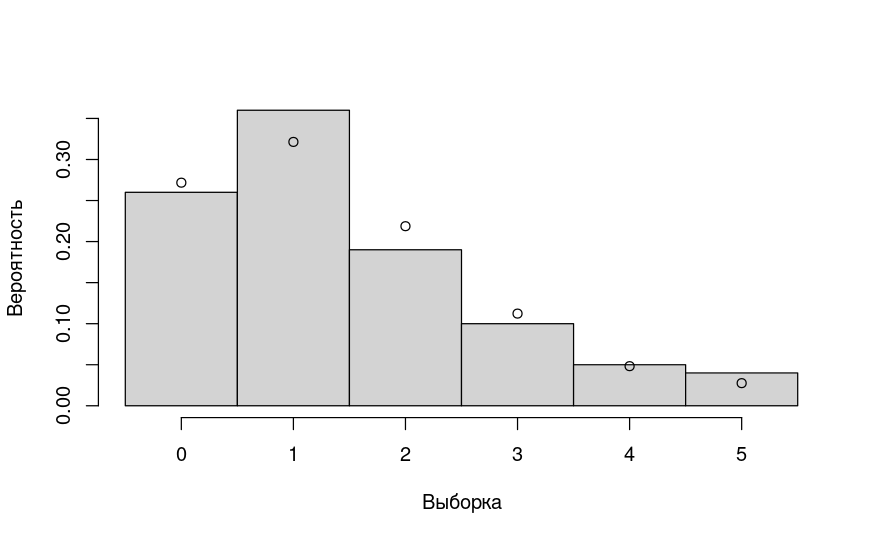
\includegraphics[width = 0.6\textwidth]{binlogexpprob}
		\caption{Эмпирические частоты (столбики) и теоретические частоты (точки), вычисленные по методу максимального правдоподобия}
		\label{img:binlogexpprob}
	\end{figure}
	
	Для нахождения параметров биномиально-логарифмического распределения можем применить метод максимального правдоподобия в общем случае (то есть для любых вероятностей), а для логарифмически-биномиального будем считать значения больше $ 4 $ одинаковыми. Составим функцию правдоподобия:
	\[
		\begin{aligned}
			\mathcal{L} (x _1, \dots, x _m, p, q, n) =& \prod \limits ^m _{t = 1} P(S _\tau = x _t, p) =\\
			=& \prod \limits ^m _{t = 1} \frac 1 {x _t!} (1 - p) ^{n - x _t} \cdot q ^{x _t} \sum \limits ^{x _t} _{j = 1} \frac {n!} {(n - j)!} c(x _t, j) (p \alpha) ^j (1 - p) ^{(x _t - j)}.
		\end{aligned}
	\] 
	Прологарифмируем:
	\[
		\begin{aligned}
			\ln \mathcal{L} (x _1, \dots, x _m, p, q, n) =& \sum \limits ^m _{t = 1} \left( -\ln x _t! + (n - x _t) \ln (1 - p) + x _t q +\right.\\
			&\left.+ \ln \left( \sum \limits ^{x _t} _{j = 1} \frac {n!} {(n - j)!} c(x _t, j) (p \alpha) ^j (1 - p) ^{(x _t - j)} \right) \right).
		\end{aligned}
	\]
	
	Для оценки параметров методом правдоподобия необходимо искать минимум (максимум)  функции, то есть применять математическую оптимизацию. С помощью метода моментов можно понизить размерность этой оценки.
	
	Применим метод моментов для биномиально-логарифмического распределения, то есть если нам известно рассеяние, то можем выразить $ p $ через $ q $:
	\[
		e (S _\tau)=\frac{\ln(1 - q) + q p}{(1-q)\ln(1 - q)} \implies p = \frac {\ln(1 - q) (1 - q) \cdot eS _\tau - \ln(1 - q)} {q}.
	\]
	А теперь для логарифмически-биномиального распределения, но для него через математическое ожидание, так как через рассеяние это не представляется возможным:
	\[
		p = -\frac {\ln(1 - q)(1 - q)} {nq} \cdot \mathsf{E} S _\tau.
	\]
	Поэтому, подставив эти выражения в функцию правдоподобия, получим функцию от двух, а не трёх параметров:
	\[
		\ln \mathcal{L} (x _1, \dots, x _m, q, n).
	\]
	
	Для нахождения оценки максимального правдоподобия необходимо продифференцировать это выражение и найти нуль производной, однако для данного случая будем оценивать параметры $ q $ и $ n $ численными методами многомерной оптимизации (функция \verb|optim| в R). Также для реальных оценок будем использовать численную оптимизацию по всем параметрам без метода моментов, чтобы увеличить точность.
	
	\begin{figure}[!ht]
		\centering
		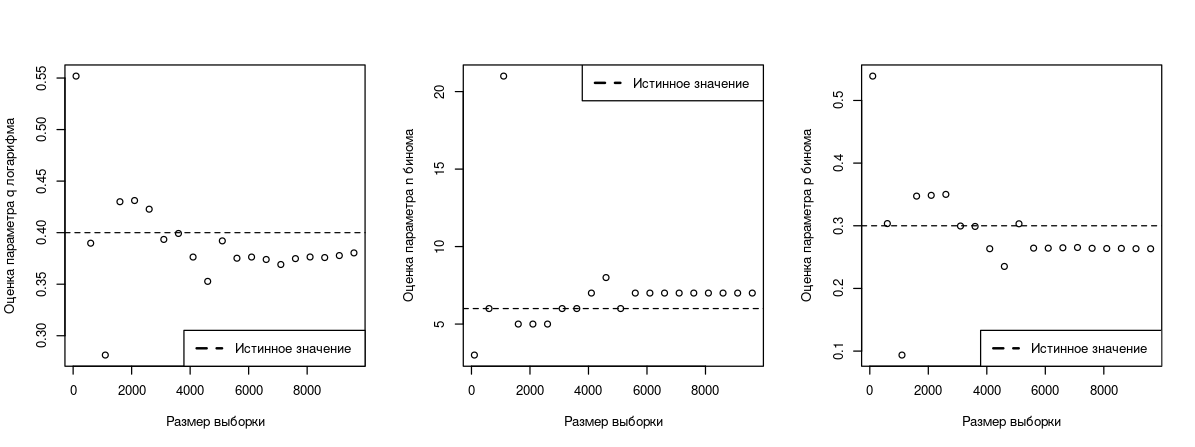
\includegraphics[width = 1\textwidth]{binomlogest}
		\caption{Сходимость оценок параметров к истинному значению для биномиально-логарифмического распределения}
		\label{img:binomlogest}
	\end{figure}
	
	\begin{figure}[!ht]
		\centering
		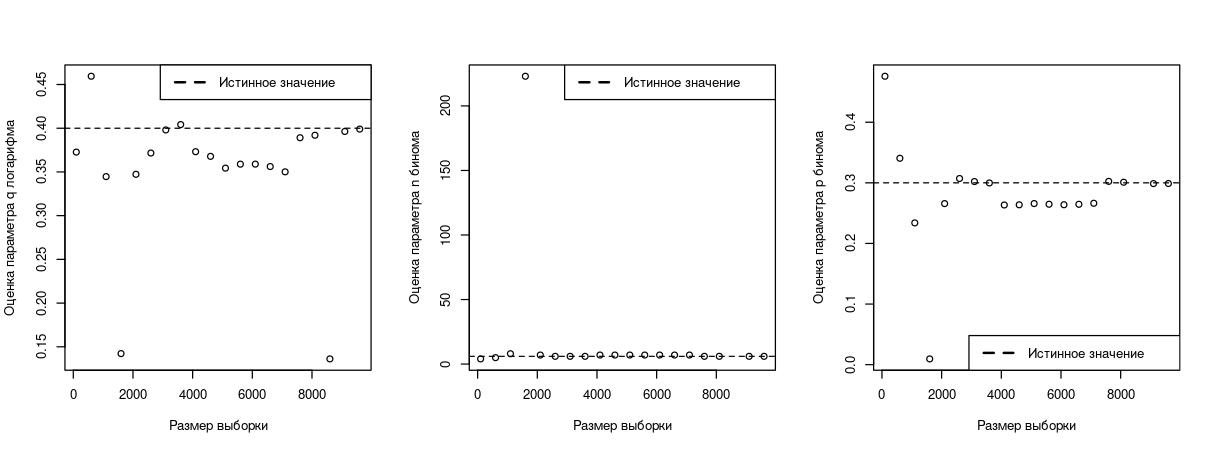
\includegraphics[width = 1\textwidth]{logbinomest}
		\caption{Сходимость оценок параметров к истинному значению для логарифмически-биномиального распределения}
		\label{img:logbinomest}
	\end{figure}

	Оценка параметра $n$ производилась методом целочисленного тернарного поиска (деление отрезка на три части и выбор из двух средних точек максимальной для сужения интервала на котором точно есть экстремум). Оценки максимального правдоподобия являются состоятельными, в чём можем убедиться моделированием (рис.~\ref{img:binomlogest} и~\ref{img:logbinomest}), хотя сходимость для данных распределений медленная из-за оценки трёх параметров одновременно, а для биномиально-логарифмического при небольшом размере выборки оценки получаются смещёнными.
	
	Например, in vitro при $ 35 $ Гр получаем наилучшие оценки: $ n = 866, q = 0.1799, p = 0.0015$. Значимость согласия по критерию $ \chi ^2 $: $ p-value = 0.26 $. Результат представлен на рис. \ref{img:binlogexpprob}.
	
	\section{Применение биномиально-логарифмического и логарифмически-биномиального распределения в радиобиологии}
	
	\label{radiobiology}
	
	\begin{table}[ht]
		\centering
		\caption*{Оценки параметров и значимости критерия хи-квадрат биномиально-логарифмического распределения.}
		\small
		\begin{minipage}{0.48\textwidth}
			\centering
			\caption{In vivo}
			
			\begin{tabular}{rrrrr}
				\hline
				Доза, Гр & n & q & p & \textbf{p-value} \\ 
				\hline
				0 & 1 & 0.20 & 0.34 & \textbf{0.99} \\ 
				5 & 6 & 1.4e-6 & 0.11 & \textbf{0.63} \\ 
				10 & 2 & 0.21 & 0.37 & \textbf{0.62} \\ 
				15 & 2 & 0.24 & 0.50 & \textbf{0.15} \\ 
				20 & 82 & 0.24 & 0.02 & \textbf{0.03} \\ 
				25 & 4 & 0.21 & 0.24 & \textbf{0.60} \\ 
				30 & 997 & 0.16 & 1.6e-3 & \textbf{0.27} \\ 
				35 & 988 & 0.03 & 1.9e-3 & \textbf{0.03} \\ 
				40 & 983 & 0.01 & 2.2e-3 & \textbf{0.09} \\
				45 & 33 & 7.0e-6 & 0.07 & \textbf{0.02} \\ 
				\hline
			\end{tabular}
			\label{tab:binomlogvivo}
		\end{minipage}
		\hfill
		\begin{minipage}{0.48\textwidth}
			\centering
			\caption{In vitro}
			
			\begin{tabular}{rrrrr}
				\hline
				Доза, Гр & n & q & p & \textbf{p-value} \\ 
				\hline
				0 & 10 & 3.9e-6 & 0.04 & \textbf{0.45} \\ 
				5 & 990 & 0.24 & 3.1e-3 & \textbf{0.84} \\ 
				10 & 960 & 0.08 & 5.7e-3 & \textbf{0.06} \\ 
				15 & 1 & 0.61 & 0.52 & \textbf{0.81} \\ 
				20 & 1 & 0.47 & 0.41 & \textbf{0.85} \\ 
				25 & 995 & 0.16 & 1.0e-3 & \textbf{0.28} \\ 
				30 & 2 & 0.47 & 0.40 & \textbf{0.77} \\ 
				35 & 866 & 0.18 & 1.5e-3 & \textbf{0.26} \\ 
				40 & 981 & 0.08 & 1.6e-3 & \textbf{0.24} \\
				\hline
			\end{tabular}
			\label{tab:binomlogvitro}
		\end{minipage}
		\label{tab:binomlog}
	\end{table}

	\begin{table}[ht]
		\centering
		\caption*{Оценки параметров и значимости критерия хи-квадрат логарифмически-биномиального распределения.}
		\small
		\begin{minipage}{0.48\textwidth}
			\centering
			\caption{In vivo}
			
			\begin{tabular}{rrrrr}
				\hline
				Доза, Гр & n & q & p & \textbf{p-value} \\ 
				\hline
				0 & 1 & 0.47 & 0.27 & \textbf{0.99} \\ 
				5 & 6 & 7.6e-7 & 0.11 & \textbf{0.63} \\ 
				10 & 20 & 4.3e-7 & 0.04 & \textbf{0.67} \\ 
				15 & 2 & 0.31 & 0.48 & \textbf{0.13} \\ 
				20 & 995 & 4.4e-6 & 1.7e-3 & \textbf{0.03} \\ 
				25 & 6 & 0.27 & 0.15 & \textbf{0.63} \\ 
				30 & 1000 & 0.32 & 1.5e-3 & \textbf{0.31} \\ 
				35 & 998 & 0.19 & 1.7e-3 & \textbf{0.11} \\ 
				40 & 1000 & 0.22 & 2.1e-3 & \textbf{0.16} \\
				45 & 998 & 0.18 & 2.3e-3 & \textbf{0.08} \\ 
				\hline
			\end{tabular}
			\label{tab:logbinomvivo}
		\end{minipage}
		\hfill
		\begin{minipage}{0.48\textwidth}
			\centering
			\caption{In vitro}
			
			\begin{tabular}{rrrrr}
				\hline
				Доза, Гр & n & q & p & \textbf{p-value} \\ 
				\hline
				0 & 20 & 1.7e-6 & 0.02 & \textbf{0.52} \\ 
				5 & 994 & 0.80 & 1.4e-4 & \textbf{0.73} \\ 
				10 & 1000 & 1.1e-6 & 5.9e-4 & \textbf{0.03} \\ 
				15 & 2 & 0.80 & 0.18 & \textbf{0.72} \\ 
				20 & 981 & 0.54 & 3.9e-4 & \textbf{0.48} \\ 
				25 & 960 & 0.37 & 9.2e-4 & \textbf{0.22} \\ 
				30 & 2 & 0.69 & 0.31 & \textbf{0.61} \\ 
				35 & 8 & 0.52 & 0.12 & \textbf{0.52} \\ 
				40 & 8 & 0.43 & 0.16 & \textbf{0.73} \\
				\hline
			\end{tabular}
			\label{tab:logbinomvitro}
		\end{minipage}
		\label{tab:logbinom}
	\end{table}

	\begin{figure}[!ht]
		\centering
		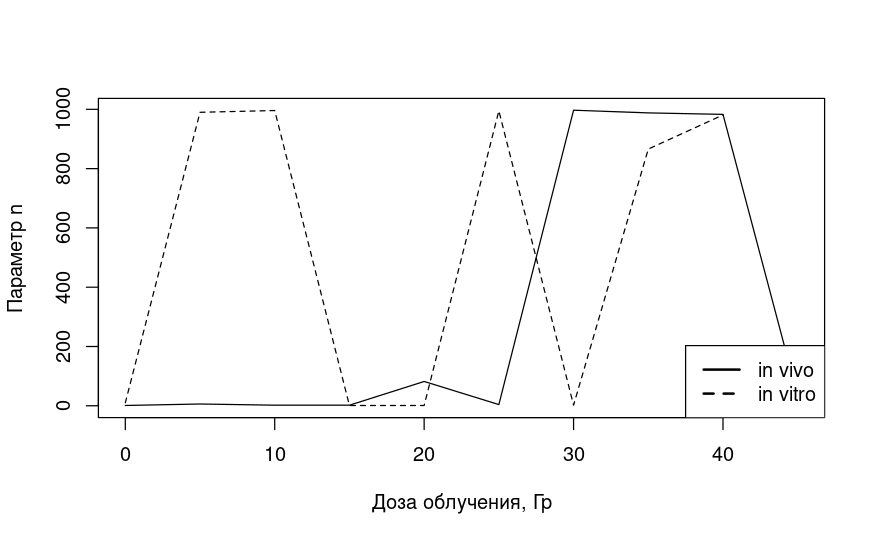
\includegraphics[width = 0.8\textwidth]{logbinomn}
		\caption{Оценка параметра $n$ для биномиально-логарифмического распределения в зависимости от дозы облучения}
		\label{img:logbinomn}
	\end{figure}
	
	При промежуточных результатах была выдвинута следующая интерпретация: $ n $ "--- экстенсивность внешнего воздействия (экстенсивность облучения), $ p $ "--- интенсивность внешнего воздействия (вероятность возникновения аномалии при облучении), $ q $ "--- инертность (вероятность развития аномалии при делении). Таким образом, наследование аномалий осуществляется по логарифмическому закону, а образование аномалий за счет облучения  по биномиальному.
	
	Однако мы применили логарифмически-биномиальное и биномиально-логарифмическое распределения к in vivo и in vitro данным одновременно. С помощью численной оптимизации трёхмерных функций правдоподобия для каждой выборки ядерных аномалий у крыс получены результаты согласованности по критерию $ \chi ^2 $, отражённые в таблицах~\ref{tab:binomlogvivo}, ~\ref{tab:binomlogvitro}, ~\ref{tab:logbinomvivo}, ~\ref{tab:logbinomvitro}.
	
	Какой либо зависимости параметров от дозы облучения заметить не удаётся. Для примера покажем график для параметра $n$ в биномиально-логарифмическом распределении (рис.~\ref{img:logbinomn}).
	
	При этом для подавляющего большинства случаев биномиально-логарифмическое ($16 / 19 \cdot 100\% = 84\%$) и логарифмически-биномиальное распределения ($17 / 19 \cdot 100\% = 89\%$) дают согласованность на уровне $\alpha = 0.05$, что, с учётом небольшого числа случаев (всего $19$) близко к теоретическим значениям.
	
	Параметры $n$ и $p$ имеют большой разброс значений и часто $n$ устремляется в бесконечность (при оценке оценка параметра ограничена $1000$), а $p$ к нулю, что приводит нас к другому сложному распределению.
	
	\section{Логарифмически-пуассоновское распределение}
	
	Логарифмически-биномиальное распределение можно свести к распределению с меньшим количеством параметров. Для этого устремим параметр $n$ к бесконечности, а $p$ к нулю так, чтобы $n \cdot p = \lambda$. По теореме Пуассона, таким образом, из биномиального распределения получается распределение Пуассона. Покажем это на примере производящей функции: 
	\[
		\begin{aligned}
			f (t) =& (p t + 1 - p) ^n = \left(1 + \frac {1}{\frac{1 - p} {pt}}\right) ^n \cdot (1 - p) ^n = \left(1 + \frac {1}{\frac{1 - p} {pt}}\right) ^{\frac{1 - p} {pt} n \frac {pt} {1 - p}} \cdot e ^{n \ln(1 - p)} \stackrel{(!)}{=}\\
			\stackrel{(!)}{=}& \left(\left(1 + \frac {1}{\frac{1 - p} {pt}}\right) ^{\frac{1 - p} {pt}}\right) ^ {n \frac {pt} {1 - p}} \cdot e ^{-np + no(p ^2)} \xrightarrow[\substack{p \to 0\\n \to \infty\\n \cdot p = \lambda}]{} e ^{\lambda (t - 1)},
		\end{aligned}
	\]
	где переход $(!)$ сделан по разложению логарифма в районе нуля в ряд Тейлора, а при устремлении параметров использован замечательный предел.
	
	Делаем аналогичный переход в производящей функции логарифмически-биномиальном распределении и получим новое распределение от $2$-х параметров.
	
	\begin{define}
		Пусть $\xi _1, \xi _2, \dots$ "--- независимые одинаково распределённые случайные величины, $\xi _i \sim Pois(\lambda), \forall i$, то есть удовлетворяют пуассоновскому закону с параметром $\lambda$, $\tau \sim Log(q)$ "--- логарифмическому закону с параметром $q$ и независима от $\xi _i, \forall i$.
		
		Тогда случайная сумма $S _\tau = \xi _1 + \dots + \xi _\tau$ будет случайной величиной, удовлетворяющей логарифмически-пуассоновскому распределению ($LogPois(q, \lambda)$ или кратко \glqq ЛПР\grqq).
		
		Суперпозиция производящих функций логарифмического и пуассоновского распределения даст производящую функцию ЛПР:
		\begin{equation}\label{eq:LPR}
			h _3 (t) = -\alpha \ln (1 - q e ^{\lambda (t - 1)})
		\end{equation}
		\label{def:LPR}
	\end{define}

	Очевидным преимуществом данного распределения является вещественность всех его параметров, а также, в принципе, их количество: два против трёх. Однако было утеряно свойство переменчивости знака логарифма рассеяния, что следует, в том числе, из леммы~\ref{lemma:1}
	
	Обозначим простейшие характеристики данного распределения:
	\[
		\begin{aligned}
			\mathsf{E} S _\tau &= \mathsf{E} \xi _i \mathsf{E} \tau = \frac {\lambda \alpha q} {1 - q},\\
			\mathsf{D} S _\tau &= \left( \mathsf{E} \xi _i \right) ^2 \mathsf{D} \tau + \mathsf{E} \tau \mathsf{D} \xi _i = \lambda \alpha q \frac {\lambda + (1 - q) - \lambda \alpha q} {(1 - q) ^2},\\
			e (S _\tau) &= \mathsf{E} \xi _i e (\tau) + e (\xi _i) = \frac {\lambda + (1 - q) - \lambda \alpha q} {1 - q}.
		\end{aligned}
	\]
	Ещё раз убеждаемся в том, что рассеяние больше $1$:
	\[
		\begin{aligned}
			\frac {\lambda q + \lambda \ln (1 - q) + (1 - q) \ln(1 - q)} {\ln(1 - q) (1 - q)} =& 1\\
			\lambda (q + \ln (1 - q)) =& 0,
		\end{aligned}
	\]
	А это справедливо только при $\lambda = 0$ или $q = 0$.
	
	\subsection{Вероятности}
	
	Вероятности находим аналогично биномиально-логарифмическому и логарифмически-биномиальному распределениям через формулу для производящих функций.

	\begin{theorem}
		\label{theorem:probLPR1}
		Вероятности логарифмически-пуассоновского распределения с параметрами $\lambda > 0$ и $q \in (0, 1)$ и производящей функцией:
		\[
		h _3 (t) = -\alpha \ln \left(1 - q e ^{\lambda (t - 1)}\right),
		\]
		равны при $k = 0$:
		\[
			P(S _\tau = 0) = -\alpha \ln\left(1 - q e ^{-\lambda}\right),
		\]
		а при $k = 1, 2 \dots$:
		\begin{equation}\label{lpr:prob1}
			P(S _\tau = k) = \frac \alpha {k !} \lambda ^k \sum \limits _{j = 1} ^{k} (j - 1)! S(k, j) \left(\frac {q e ^{-\lambda}} {1 - q e ^{-\lambda}}\right) ^j,
		\end{equation}
		где $S(k, j)$ "--- числа Стирлинга второго рода~\cite{bib:knuth1998}, имеющие следующую рекуррентную формулу:
		\[
			S(k, j) = S(k - 1, j - 1) + j \cdot S(k - 1, j), \quad 0 < j \leqslant k,
		\]
		\[
			S(0, 0) = 1, S(n, 0) = 0~ \text{при}~ n > 0, S(k, j) = 0~ \text{при}~ j > k.
		\]
	\end{theorem}

	\begin{proof}[Доказательство]
		Вероятность для $k = 0$ получается простой подстановкой нуля в производящую функцию.
		
		Для доказательство остальных значений $k$ воспользуемся методом математической индукции:
		
		\begin{enumerate}
			\item Докажем для $k = 1$:
			\[
				\begin{aligned}
					P (S _\tau = 1) =& \left.\frac 1 {1 !} \left(h _3(t)\right)'\right| _{t = 0} = \left.\left(-\alpha \ln \left(1 - q e ^{\lambda (t - 1)}\right)\right)'\right| _{t = 0} = \left.-\alpha \frac {-q \lambda e ^{\lambda (t - 1)}} {1 - q e ^{\lambda (t - 1)}} \right| _{t = 0} =\\
					=& \alpha \lambda \frac {q e ^{-\lambda}} {1 - q e ^{-\lambda}},
				\end{aligned}
			\]
			что соответствует формуле~\ref{lpr:prob1} при подстановке в неё $k = 1$.
			
			\item Докажем переход от $k$ к $k + 1$.
			
			Для этого обозначим $q e ^{\lambda (t - 1)} = m$ и заметим, что $m' = \left(q e ^{\lambda(t - 1)}\right)' = \lambda q e ^{\lambda(t - 1)} = \lambda m $.
			
			Уже доказано, что
			\[
				h _3 ^{(k)} (t) = \alpha \lambda ^k \sum \limits _{j = 1} ^{k} (j - 1)! S(k, j) \left(\frac m {1 - m}\right) ^j
			\]
			(это выражение зависит от $t$, но достаточно в первом пункте при $k = 1$ не подставлять $t = 0$, чтобы база математической индукции была верна). Докажем, что
			\[
				h _3 ^{(k + 1)} (t) = \alpha \lambda ^{k + 1} \sum \limits _{j = 1} ^{k + 1} (j - 1)! S(k + 1, j) \left(\frac m {1 - m}\right) ^j.
			\]
			Это следует из цепочки равенств:
			\[
				\begin{aligned}
					&\left(\lambda ^k \sum \limits _{j = 1} ^{k} (j - 1)! S(k, j) \left(\frac m {1 - m}\right) ^j\right)' =\\
					&\quad= \lambda ^k \sum \limits _{j = 1} ^{k} (j - 1)! S(k, j) j \left(\frac m {1 - m}\right) ^{j - 1} \cdot \left(\frac {\lambda m} {1 - m} + \frac {\lambda m ^2} {(1 - m) ^2}\right) =\\
					&\quad= \lambda ^{k + 1} \left(\sum \limits _{j = 1} ^{k} j! S(k, j) \left(\frac m {1 - m}\right) ^j + \sum \limits _{j = 1} ^{k} j! S(k, j) \left(\frac m {1 - m}\right) ^{j + 1}\right) =\\
					&\quad= \lambda ^{k + 1} \left(\sum \limits _{j = 1} ^{k} j! S(k, j) \left(\frac m {1 - m}\right) ^j + \sum \limits _{j = 2} ^{k + 1} (j - 1)! S(k, j - 1) \left(\frac m {1 - m}\right) ^j\right) =\\
					&\quad= \lambda ^{k + 1} \left(S(k, 1) \frac m {1 - m} +\right.\\
					&\quad~~ + \sum \limits _{j = 2} ^{k} \left(j! S(k, j) \left(\frac m {1 - m}\right) ^j + (j - 1)! S(k, j - 1) \left(\frac m {1 - m}\right) ^j\right) +\\
					&\quad~~ \left.+ k ! S (k, k) \left(\frac m {1 - m}\right) ^{k + 1}\right) =\\
					&\quad= \lambda ^{k + 1} \left(S(k + 1, 1) \frac m {1 - m} + \sum \limits _{j = 2} ^{k} (j - 1)! \left(j S(k, j) + S(k, j - 1)\right) \left(\frac m {1 - m}\right) ^j +\right.\\
					&\quad~~\left.+ k ! s (k + 1, k + 1) \left(\frac m {1 - m}\right) ^{k + 1}\right) =\\
				\end{aligned}
			\]
			\[
				\begin{aligned}
					&\quad= \lambda ^{k + 1} \left(S(k + 1, 1) \frac m {1 - m} + \sum \limits _{j = 2} ^{k} (j - 1)! S(k + 1, j) \left(\frac m {1 - m}\right) ^j +\right.\\
					&\quad~~\left.+ k ! s (k + 1, k + 1) \left(\frac m {1 - m}\right) ^{k + 1}\right) =\\
					&\quad=\lambda ^{k + 1} \sum \limits _{j = 1} ^{k + 1} (j - 1)! S(k + 1, j) \left(\frac m {1 - m}\right) ^j
				\end{aligned}
			\]
			Заметим, что $S(l, 1) = 1~ \forall l > 0$ и $S(m, m) = 1~ \forall m \geqslant 0$, поэтому замены $S(k, 1)$ на $S(k + 1, 1)$ и $S(k, k)$ на $S(k + 1, k + 1)$ легитимные.
			
			Коэффициент $\alpha$ не влияет на дифференцирование, а также $q e ^{-\lambda} = m | _{t = 0}$, поэтому переход доказан.
		\end{enumerate}
	\end{proof}

	Полученная формула имеет связь с числами Стирлинга второго рода, которые обозначают количество неупорядоченных разбиений $k$-элементного множества на $j$ непустых подмножеств. В разделе~\ref{sec:probBLR} была показана формула для вероятности через числа Стирлинга первого рода, что говорит о том, что данные числа могут иметь большую важность для различных классов сложных распределений. 
	
	Явная формула для чисел Стирлинга:
	\[
	S(k, j) = \frac {1} {j!} \sum \limits _{i = 0} ^j (-1) ^{j + i} C _{j} ^{i} i ^k.
	\]
	И приведём небольшую часть таблицы чисел Стирлинга (таб.~\ref{tab:stirling2}).
	\begin{table}[!h]
		\centering
		\caption{Числа Стирлинга второго рода}
		\begin{tabular}{c|ccccccc}
			$k$ \textbackslash $j$ & $0$ & $1$ & $2$ & $3$ & $4$ & $5$ & $6$\\ \hline
			$0$ & $1$ &   &  &  & &  &\\
			$1$ & $0$ & $1$ &  &  & &  &\\
			$2$ & $0$ & $1$ & $1$ &  & &  &\\
			$3$ & $0$ & $1$ & $3$ & $1$ &  & &\\
			$4$ & $0$ & $1$ & $7$ &  $6$ & $1$ & & \\
			$5$ & $0$ & $1$ & $15$ & $25$ & $10$ & $1$ & \\
			$6$ & $0$ & $1$ & $31$ & $90$ & $65$ & $15$ & $1$
		\end{tabular}
		\label{tab:stirling2}
	\end{table}
	
	Для логарифмически-пуассоновского распределения можно получить формулу другого вида с другим классом чисел.
	
	\begin{theorem}
		\label{theorem:probLPR2}
		В условиях теоремы~\ref{theorem:probLPR1} вероятности логарифмически-пуассоновского распределения могут быть выражены следующим образом:
		\begin{enumerate}
			\item Для $k = 0, 1$ формула аналогична теореме~\ref{theorem:probLPR1};
			
			\item Для $k = 2, ...$:
			\begin{equation}\label{lpr:prob2}
				P(S _\tau = k) = \frac \alpha {k !} \frac {\lambda ^k q e ^{-\lambda}} {\left(1 - q e ^{-\lambda}\right) ^k} \sum \limits _{j = 0} ^{k - 2} E(k - 1, j) \left(q e ^{-\lambda}\right) ^j, 
			\end{equation}
			где $E(k, j)$ "--- числа Эйлера первого рода~\cite{bib:knuth1998}. Они имеют следующую рекуррентную формулу:
			\[
				E(k, j) = (j + 1) \cdot E(k - 1, j) + (k - j) \cdot E(k - 1, j - 1), 0 < j < k - 1,
			\]
			\[
				E(k, 0) = 1~ \text{при}~ k \geqslant 0, E(k, j) = 0~ \text{при}~ j \geqslant k > 0.
			\]
		\end{enumerate}
	\end{theorem}
	
	\begin{proof}[Доказательство]
		Формулы для $k = 0, 1$ получены аналогично теореме~\ref{theorem:probLPR1}.
		
		Проведём математическую индукцию для остальных значений $k$. Сразу применим замену $m = q e ^{\lambda(t - 1)}$.
		
		\begin{enumerate}
			\item База индукции:
			\[
				\begin{aligned}
					P (S _\tau = 2) =& \left.\frac 1 {2 !} \left(h _3(t)\right)''\right| _{t = 0} = \left.\left(-\alpha \ln \left(1 - m \right)\right)''\right| _{t = 0} = \left.\frac 1 2 \left(-\alpha \frac {-\lambda m} {1 - m}\right)' \right| _{t = 0} =\\
					=&  \left.\frac \alpha 2 \lambda \frac {\lambda m \left(1 - m\right) - m \left(-\lambda m\right)} {\left(1 - m\right) ^2}\right| _{t = 0} = \frac \alpha 2 \frac {\lambda ^2 q e ^{-\lambda}} {\left(1 - q e ^{-\lambda}\right) ^2},
				\end{aligned}
			\]
			
			\item Докажем переход от $k$ к $k + 1$.
			
			Уже доказано, что
			\[
			h _3 ^{(k)} (t) = \alpha \frac {\lambda ^k q e ^{-\lambda}} {(1 - m) ^k} \sum \limits _{j = 0} ^{k - 2} E(k - 1, j) m ^j
			\]
			(это выражение зависит от $t$, но достаточно в первом пункте при $k = 1$ не подставлять $t = 0$, чтобы база математической индукции была верна). Докажем, что
			\[
			h _3 ^{(k + 1)} (t) = \alpha \frac {\lambda ^{k + 1} m} {(1 - m) ^{k + 1}} \sum \limits _{j = 0} ^{k - 1} E(k, j) m ^j.
			\]
			Это следует из следующей цепочки:
			\[
				\begin{aligned}
					&\left(\frac {\lambda ^k} {(1 - m) ^k} \sum \limits _{j = 0} ^{k - 2} E(k - 1, j) m ^{j + 1}\right)' =\\
					&\quad = \frac {km\lambda ^{k + 1}} {(1 - m) ^{k + 1}} \sum \limits _{j = 0} ^{k - 2} E(k - 1, j) m ^{j + 1} + \frac {(1 - m)\lambda ^k} {(1 - m) ^{k + 1}} \sum \limits _{j = 0} ^{k - 2} E(k - 1, j) \lambda (j + 1) m ^{j + 1} =\\
					&\quad = \frac {\lambda ^{k + 1}} {(1 - m) ^{k + 1}} \cdot \left(\sum \limits _{j = 0} ^{k - 2} E(k - 1, j) k m ^{j + 2} + \sum \limits _{j = 0} ^{k - 2} E(k - 1, j) (j + 1) m ^{j + 1} -
					\right.\\
					&\quad~~\left. - \sum \limits _{j = 0} ^{k - 2} E(k - 1, j) (j + 1) m ^{j + 2}\right) =\\
					&\quad = \frac {\lambda ^{k + 1}} {(1 - m) ^{k + 1}} \cdot \Bigg(E(k - 1, 0) m +\\
					&\quad~~ + \sum \limits _{j = 1} ^{k - 2} \left(E(k - 1, j) (j + 1) +E(k - 1, j - 1) (k - j)\right) m ^{j + 1} +\\
					&\quad~~ + E(k - 1, k - 2) m ^k\Bigg) =\\
					&\quad = \frac {\lambda ^{k + 1}} {(1 - m) ^{k + 1}} \left(E(k, 0) m + \sum \limits _{j = 1} ^{k - 2} E(k, j) m ^j + E(k, k - 1) m ^k \right) =\\
					&\quad = \frac {\lambda ^{k + 1}} {(1 - m) ^{k + 1}} \sum \limits _{j = 0} ^{k - 1} E(k, j) m ^{j + 1} = \frac {\lambda ^{k + 1} m} {(1 - m) ^{k + 1}} \sum \limits _{j = 0} ^{k - 1} E(k, j) m ^j
				\end{aligned}
			\]
			Заметим, что $E(l, 0) = 1~ \forall l \geqslant 0$ и $E(m, m - 1) = 1~ \forall m \geqslant 1$, поэтому замены $E(k - 1, 0)$ на $E(k, 0)$ и $E(k - 1, k - 2)$ на $E(k, k - 1)$ легитимные.
			
			Подставляем $t = 0$, умножаем на $\alpha / (k + 1)!$ и получаем нужную формулу.
		\end{enumerate}
	\end{proof}

	Числа Эйлера представляют собой количество перестановок порядка $k$ с $j$ подъёмами, то есть в перестановке $\pi = (\pi _1, \dots, \pi _k)$ всего $j$ индексов $i$ таких, что $\pi _i < \pi _{j + 1}$. Приведём небольшую часть таблицы чисел Эйлера (таб.~\ref{tab:eiler1}).

	\begin{table}[!ht]
		\centering
		\caption{Числа Эйлера первого рода}
		\begin{tabular}{c|cccccc}
			$k$ \textbackslash $j$ & $0$ & $1$ & $2$ & $3$ & $4$ & $5$\\ \hline
			$0$ & $1$ &  &  &  &  & \\
			$1$ & $1$ &  &  &  &  & \\
			$2$ & $1$ & $1$ &  &  &  & \\
			$3$ & $1$ & $4$ & $1$ &  &  & \\
			$4$ & $1$ & $11$ & $11$ & $1$ &  & \\
			$5$ & $1$ & $26$ & $66$ & $26$ & $1$ & \\
			$6$ & $1$ & $57$ & $302$ & $302$ & $57$ & $1$ \\
		\end{tabular}
		\label{tab:eiler1}
	\end{table}

	Для них можно привести явную формулу:
	\[
		E(k, j) = \sum \limits ^j _{i = 0} C ^i _{k + 1} (-1) ^i (j + 1 - i) ^k.
	\]

	Эти числа также возникают в следующих бесконечных функциональных рядах:
	\[
		\sum \limits ^\infty _{i = 1} i ^k x ^i = \frac {x} {(1 - x) ^{k + 1}} \sum \limits ^{k - 1} _{j = 0} E(k, j) x ^j.
	\]
	Поэтому можно убедиться в справедливости формул вероятностей из теоремы~\ref{theorem:probLPR2}. Используем формулу полной вероятности, чтобы найти вероятность случайной суммы случайных величин:
	\[
		\begin{aligned}
			P(S _\tau = k) =& \sum \limits ^{\infty} _{j = 1} P(\left.S _\tau = k\right| \tau = j) \cdot P(\tau = j) = \sum \limits ^{\infty} _{j = 1} - \frac 1 {\ln(1 - q)} \frac {q ^j} j \cdot P(\xi _1 + \dots + \xi _j = k) =\\
			=& \sum \limits ^{\infty} _{j = 1} - \frac 1 {\ln(1 - q)} \frac {q ^j} j \frac {(j \lambda) ^k} {k !} e ^{-j \lambda} = \frac \alpha {k !} \lambda ^k \sum \limits ^{\infty} _{j = 1} j ^{k - 1} \left(q e ^{-\lambda}\right) ^j =\\
			=& \frac \alpha {k !} \frac {\lambda ^k q e ^{-\lambda}} {\left(1 - q e ^{-\lambda}\right) ^k} \sum \limits ^{k - 2} _{j = 0} E(k - 1, j) \left(q e ^{-\lambda}\right) ^j.
		\end{aligned}
	\]
	
	
	Компьютерное вычисление вероятностей показало эквивалентность этих трёх формул с погрешностью на уровне машинного нуля.
	
	\subsection{Оценка параметров}
	
	\begin{figure}[!ht]
		\centering
		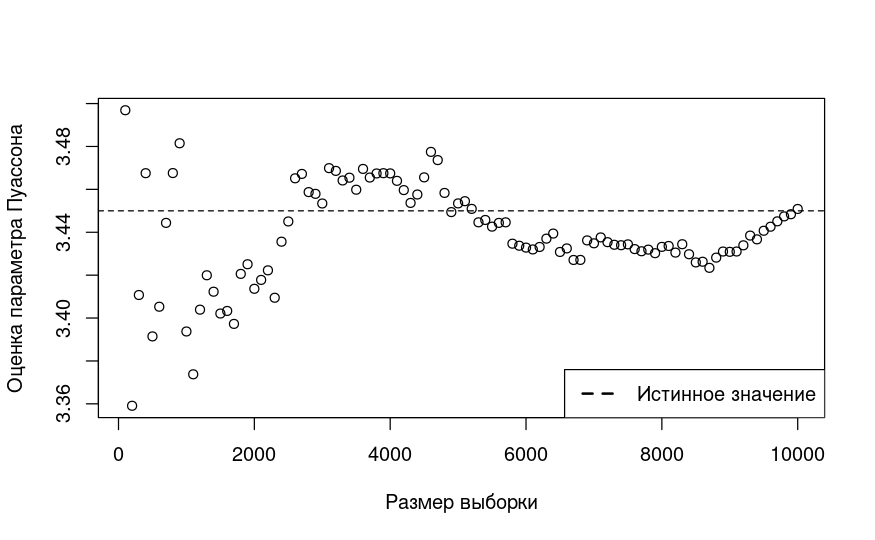
\includegraphics[width = 0.8\textwidth]{logpoislambda}
		\caption{Сходимость оценки параметра $\lambda$ к истинному значению для логарифмически-пуассоновского распределения}
		\label{img:logpoislambda}
	\end{figure}
	
	\begin{figure}[!ht]
		\centering
		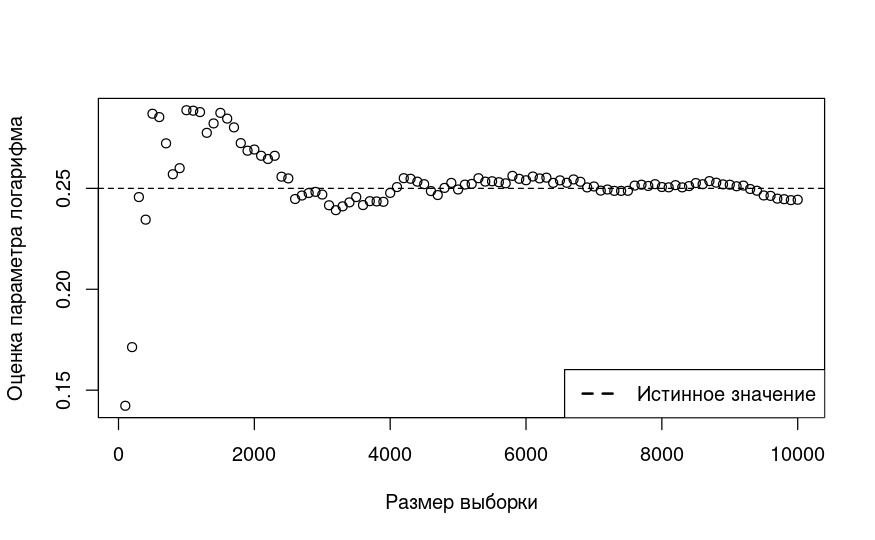
\includegraphics[width = 0.8\textwidth]{logpoisq}
		\caption{Сходимость оценки параметра $q$ к истинному значению для логарифмически-пуассоновского распределения}
		\label{img:logpoisq}
	\end{figure}
	
	Оценка параметров $\lambda$ и $q$ проводилась методом максимального правдоподобия численно на компьютере с использованием функции \verb|optim| на языке \verb|R|.
	
	Моделируя выборку из $n$ индивидов для известных параметров можно проверить состоятельность такой оценки.

	По рис.~\ref{img:logpoislambda} и~\ref{img:logpoisq} видим, что состоятельность имеет место для данных оценок.
	
	\subsection{Логарифмически-пуассоновское распределение в радиобиологии}
	
	\begin{table}[ht]
		\centering
		\caption*{Оценки параметров и значимости критерия хи-квадрат по данным in vivo и in vitro для логарифмически-пуассоновского распределения.}
		\begin{minipage}{0.4\textwidth}
			\centering
			\caption{In vivo}
			
			\begin{tabular}{rrrr}
				\hline
				Гр & $\lambda$ & $q$ & \textbf{p-v} \\ 
				\hline
				0 & 0.38 & 5.9e-7 & \textbf{0.13} \\ 
				5 & 0.67 & 3.3e-7 & \textbf{0.81} \\ 
				10 & 0.83 & 6.7e-7 & \textbf{0.21} \\ 
				15 & 1.15 & 5.3e-7 & \textbf{0.01} \\ 
				20 & 1.71 & 1e-5 & \textbf{0.03} \\ 
				25 & 1.04 & 0.07 & \textbf{0.55} \\ 
				30 & 1.48 & 0.33 & \textbf{0.33} \\ 
				35 & 1.75 & 0.19 & \textbf{0.11} \\ 
				40 & 2.05 & 0.22 & \textbf{0.16} \\
				45 & 2.36 & 0.18 & \textbf{0.08} \\ 
				\hline
			\end{tabular}
			\label{tab:logpoisvivo}
		\end{minipage}
		\begin{minipage}{0.4\textwidth}
			\centering
			\caption{In vitro}
			
			\begin{tabular}{rrrr}
				\hline
				Гр & $\lambda$ & $q$ & \textbf{p-v} \\ 
				\hline
				0 & 0.39 & 3.7e-6 & \textbf{0.59} \\ 
				5 & 0.14 & 0.80 & \textbf{0.73} \\ 
				10 & 0.59 & 1.1e-7 & \textbf{0.03} \\ 
				15 & 0.41 & 0.76 & \textbf{0.36} \\ 
				20 & 0.37 & 0.56 & \textbf{0.45} \\ 
				25 & 0.88 & 0.37 & \textbf{0.22} \\ 
				30 & 0.78 & 0.53 & \textbf{0.26} \\ 
				35 & 1.10 & 0.43 & \textbf{0.43} \\ 
				40 & 1.46 & 0.29 & \textbf{0.38} \\ 
				\hline
			\end{tabular}
			\label{tab:logpoisvitro}
		\end{minipage}
	\end{table}
	
	Как уже было сказано выше, логарифмически-биномиальное распределение давало хорошую согласованность для радиобиологических данных в случае in vivo и in vitro, однако его функция максимального правдоподобия имела неоднозначный минимум, представленный <<оврагом>>, на котором параметры $n$ и $p$ уходили в бесконечность и к нулю, соответственно. Поэтому логично, что согласованность логарифмически-пуассоновского распределения будет схожа (таблицы~\ref{tab:logpoisvivo} и \ref{tab:logpoisvitro}), однако из-за потери переменчивости знака логарифма рассеяния появился один дополнительный случай ($15$ Гр. in vivo), где p-value меньше уровня значимости.

	\subsection{Интерпретация}
	
	\begin{figure}[!ht]
		\centering
		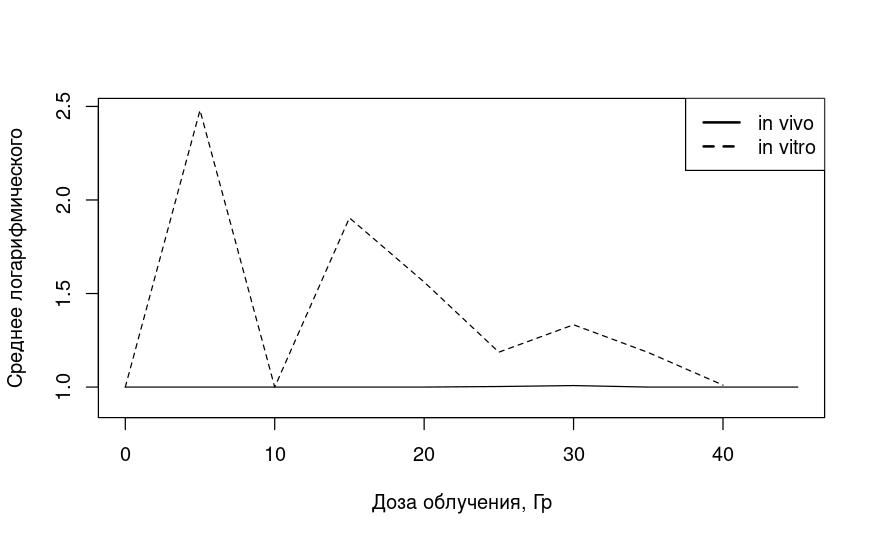
\includegraphics[width = 0.8\textwidth]{logpoismeanlog}
		\caption{Среднее логарифма в логарифмически-пуассоновском распределении в зависимости от дозы облучения}
		\label{img:logpoismeanlog}
	\end{figure}
	
	\begin{figure}[!ht]
		\centering
		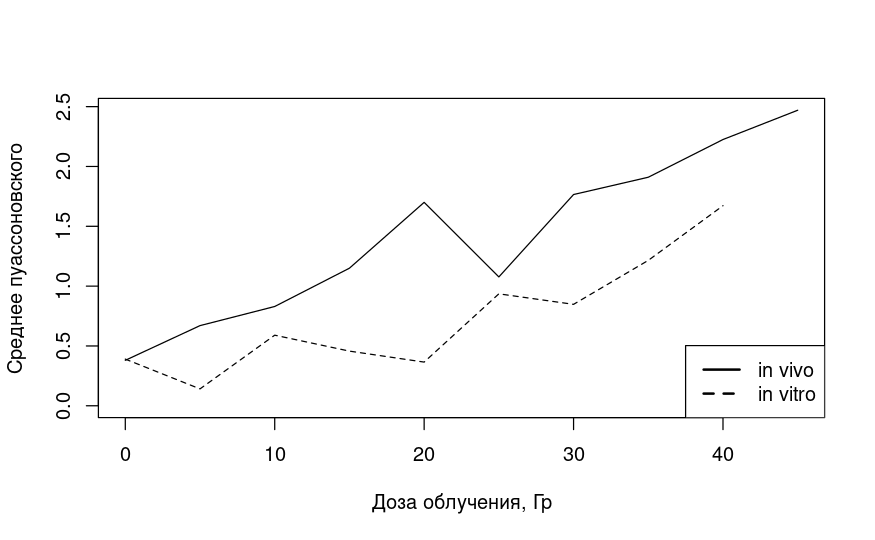
\includegraphics[width = 0.8\textwidth]{logpoismeanpois}
		\caption{Среднее Пуассона в логарифмически-пуассоновском распределении в зависимости от дозы облучения}
		\label{img:logpoismeanpois}
	\end{figure}

	Наблюдаемое количество аномалий определяется в целом двумя факторами: их исходной распространенностью и интенсивностью их образования в процессе митоза. За увеличение исходной  распространенности отвечает параметр $q$ логарифмического распределения, а за интенсивность образования аномалий в процессе митоза параметр $\lambda$  пуассоновского распределения. Поскольку распределения  суммы и самих случайных величин однопараметрические, при интерпретации  параметров можно опираться на их средние значения.
	
	Динамика оценок параметра $\lambda$,  соответственно средних значений, свидетельствует о положительной линейной зависимости их от дозы облучения, что очевидно, и о значимо меньших значениях в эксперименте in vitro (рис.~\ref{img:logpoismeanpois}), так как выжившие клетки очевидно обладают большим иммунитетом. 
	
	Что касается исходной распространенности аномалий, то, согласно динамике оценок параметра $q$  в зависимости от дозы облучения (рис.~\ref{img:logpoismeanlog}), зависимости от дозы облучения нет, а в эксперименте in vivo базовая распространенность практически не выражена и существенно меньше, чем в эксперименте in vitro. Это объясняется тем, что от дозы облучения зависит только количество выживших клеток, а не распространенность их аномалий, которая, судя по графику,   очень вариабельна, но существенно выше базовой распространенности до начала эксперимента.
	
	\chapter{Применение к анализу встречаемости слов}
	
	\label{textanalysis}
	
	\section{Постановка задачи}
	
	Для грамотного построения речевых нейросетей немаловажным является знание о распределении встречаемости слов в тексте. Хотелось бы найти такую модель (или набор моделей), которая отвечала бы всевозможным типам слов, какими бы они ни были. Сначала формализуем данную задачу.
	
	Дан текст из $ n $ глав. Некоторое слово $ \omega _j $ встречается в $ i $-ой главе $ x ^{(j)} _i $ раз. Вопрос: какому распределению удовлетворяет выборка $ (x ^{(j)} _1, \dots, x ^{(j)} _n) $?
	
	В работе~\cite{bib:alexeeva2013} утверждается, что неплохое согласование даёт модель отрицательного бинома. Однако есть ряд слов, не согласующихся с отрицательно-биномиальным распределением, поэтому возникает идея проверить их согласованность с биномиально-логарифмическим, как обобщением отрицательно-биномиального. По крайней мере, если отрицательно-биномиальное распределение даёт хорошую согласованность, то и биномиально-логарифмическое должно давать похожий результат.
	
	\section{Применение различных моделей к анализу текста}
	
	В качестве исследуемого объекта был взят роман американского писателя Теодора Драйзера \glqq Американская трагедия\grqq~ на английском языке. С помощью самописной программы получены выборки частот встречаемости слов по главам, которых в данном произведении $ 102 $ ($ n $). Всего оказалось $ 14134 $ ($ \omega_j,~ j \in \overline{1:14134} $) различных слов, однако большая их часть встречается не более $ 5 $--$ 6 $ раз во всём тексте. Поэтому будем рассматривать первые (по общему количеству во всём тексте) $ 1000 $ слов.
	
	Насчёт вычисления вероятностей: каждая из них является суммой произведений некоторого факториала, делённого на меньший факториал, чисел Стирлинга и чисел меньше единицы в степени, зависящей от индекса в сумме. Получается, что мы оперируем крайне быстро растущими и убывающими функциями, что сказывается на погрешности вычисления. Например, число Стирлинга $ 50 $-ой степени имеет $ 63 $-ий порядок. Всё это не даёт использовать в практических вычислениях биномиально-логарифмическое распределение для всевозможных эмпирических распределений без какой-то существенной модификации.
	
	\subsection{Нормированные числа Стирлинга первого рода}
	
	Для борьбы с вычислительными проблемами введём понятие нормированных чисел Стирлинга первого рода.
	
	\begin{define}
		Нормированными числами Стирлинга первого рода будем называть числа, получаемые следующим образом:
		
		\[
			l(k, j) = \frac {s(k, j)} {k!}
		\]
		\label{def:3}
	\end{define}
	
	То есть они являются числами Стирлинга первого рода, делёнными на факториал числа элементов перестановок (то есть $ k $).
	
	Выведем рекуррентную формулу для полученных чисел:
	
	\[
		\begin{aligned}
			s(k, j) =& s(k - 1, j - 1) + (k - 1) \cdot s(k - 1, j) \quad | : (k!)\\
			\frac {s(k, j)} {k!} =& \frac {s(k - 1, j - 1)} {k !} + \frac {(k - 1) \cdot s(k - 1, j)} {k !}\\
			l(k, j) =& \frac {1} {k} l(k - 1, j - 1) + \frac {(k -1)} {k} l(k - 1, j).
		\end{aligned}
	\]
	
	Так как числа Стирлинга первого рода обозначают количество перестановок длины $k$ с $j$ циклами, то сумма по строчкам должна быть равна $k!$, а значит, сумма по строчкам у нормированных чисел Стирлинга равна $1$. Приведём часть таблицы (таб.~\ref{tab:normstirling1}).
	\begin{table}[!ht]
		\centering
		\caption{Нормированные числа Стирлинга первого рода}
		\begin{tabular}{c|ccccccc}
			$k$ \textbackslash $j$ & $0$ & $1$ & $2$ & $3$ & $4$ & $5$ & $6$\\ \hline
			$0$ & $1$ &  &  &  &  &  & \\
			$1$ & $0$ & $1$ &  &  &  &  & \\
			$2$ & $0$ & $1 / 2$ & $1 / 2$ &  &  &  & \\
			$3$ & $0$ & $1 / 3$ & $1 / 2$ & $1 / 6$ &  &  & \\
			$4$ & $0$ & $1 / 4$ & $11 / 24$ & $1 / 4$ & $1 / 24$ &  & \\
			$5$ & $0$ & $1 / 5$ & $5 / 12$ & $7 / 24$ & $1 / 12$ & $1 / 120$ & \\
			$6$ & $0$ & $1 / 6$ & $137 / 360$ & $5 / 16$ & $17 / 144$ & $1 / 48$ & $1 / 720$\\
		\end{tabular}
		\label{tab:normstirling1}
	\end{table}
	
	\subsection{Оценки и согласованность}
	
	\begin{figure}[ht]
		\centering
		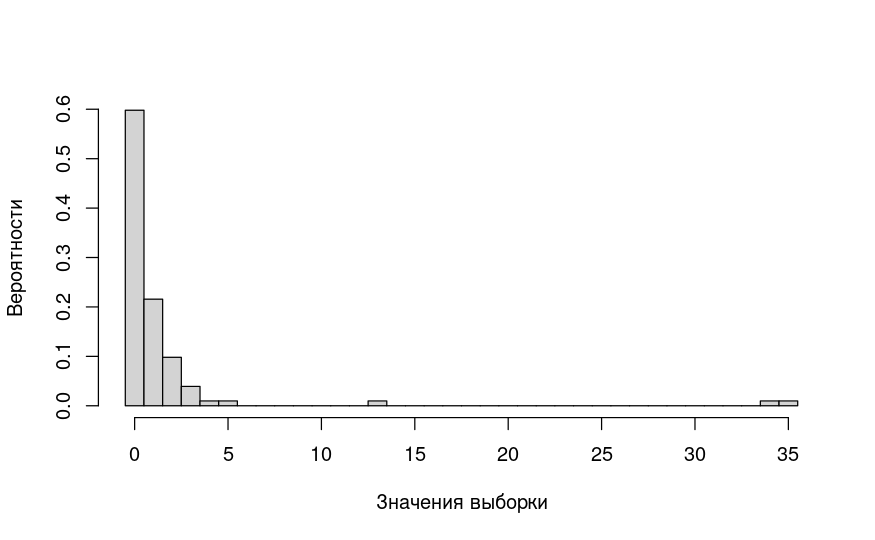
\includegraphics[width = 0.8\textwidth]{coathist}
		\caption{Гистограмма распределения слова "сoat"}
		\label{img:coathist}
	\end{figure}

	\begin{table}[t]
		\centering
		\caption{Разбиение слов по классам согласованности}
		\begin{tabular}{l|l}
			Распределение 		   & Согласованные слова \\
			\hline
			ОБР                    & 1               \\
			БЛР                    & 7               \\
			Сумма                  & 6              \\
			ОБР и БЛР              & 25              \\
			ОБР и сумма            & 4              \\
			БЛР и сумма            & 18              \\
			Все                    & 884             \\
			\hline
			Итого                  & 945          
		\end{tabular}
		\label{tab:wordclass}
	\end{table}

	\begin{figure}[!ht]
		\centering
		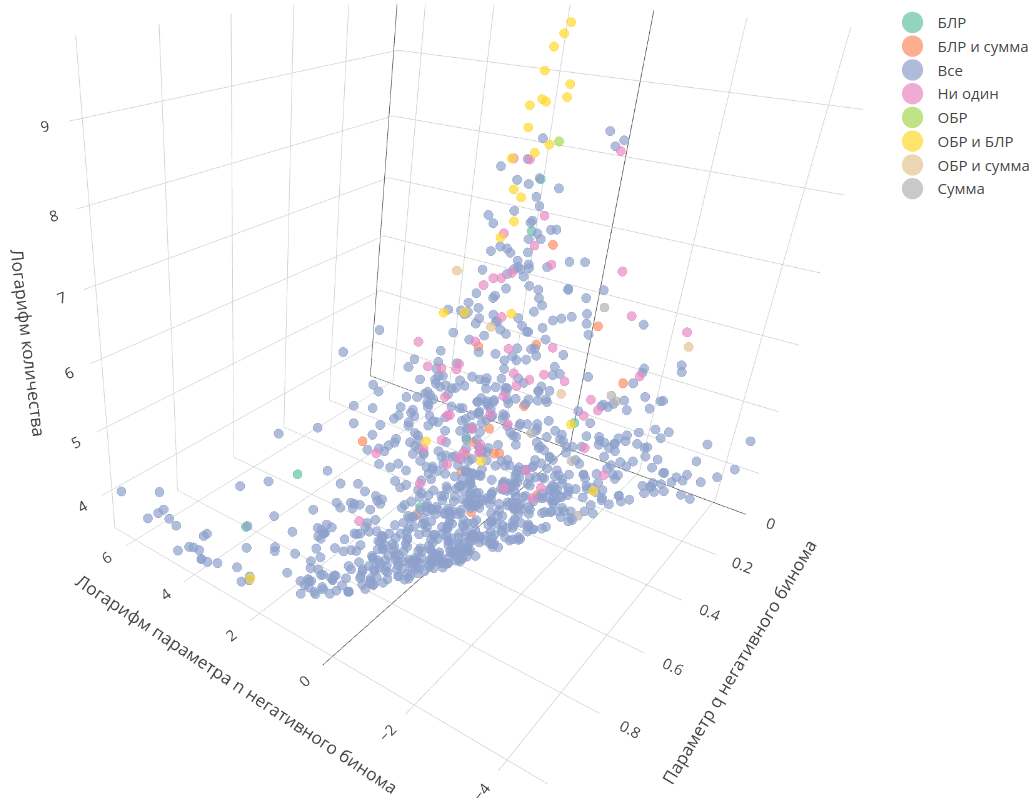
\includegraphics[width = 0.8\textwidth]{wordclassmain}
		\caption{Точечный график слов по параметрам ОБР и встречаемости, разбитые по классам.}
		\label{img:wordclassmain}
	\end{figure}
	
	\begin{figure}[!ht]
		\centering
		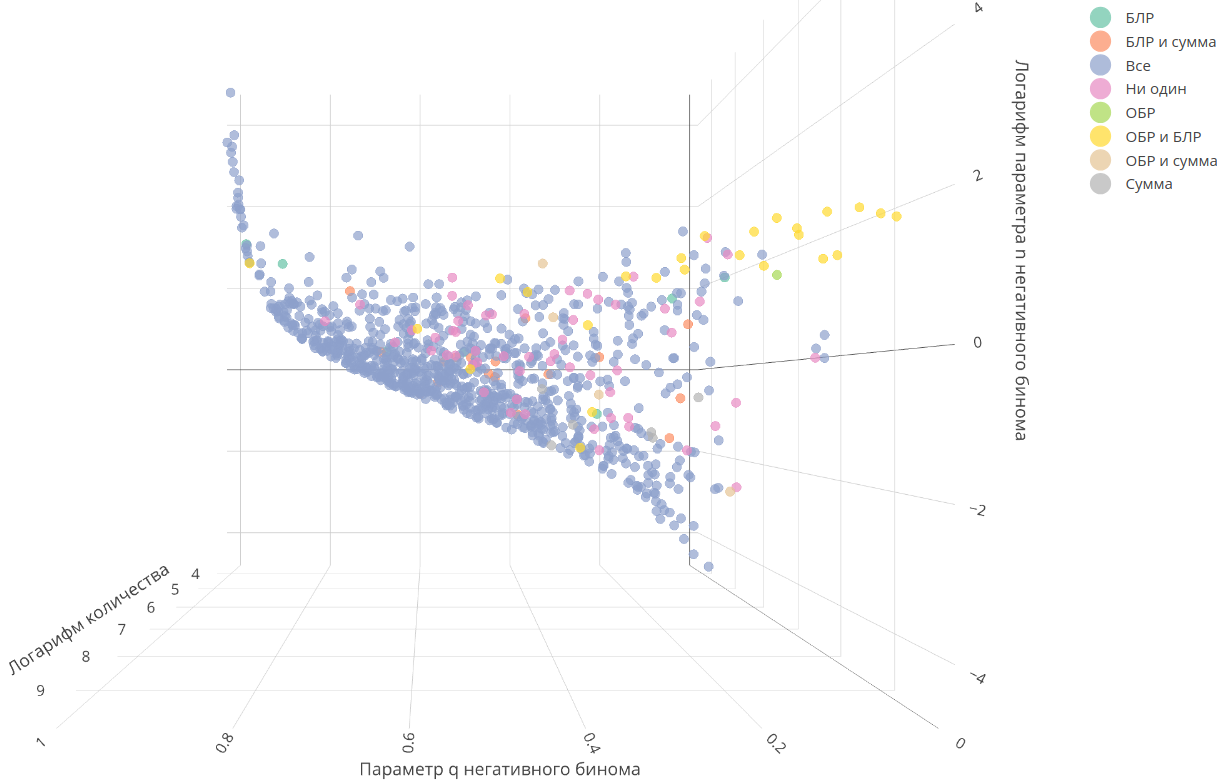
\includegraphics[width = 0.8\textwidth]{wordclassup}
		\caption{Точечный график слов по параметрам ОБР и встречаемости, разбитые по классам.}
		\label{img:wordclassup}
	\end{figure}

	Изначально в качестве моделей встречаемости слов были взяты отрицательный бином и биномиально-логарифмическое распределение, однако основная часть слов, для которой не было достигнуто согласование "--- это слова, распределение которых имеет \glqq тяжёлый\grqq~ правый хвост, выражающийся в элементах выборки, которые имеют значение встречаемости сильно больше остальных. Пример такого слова представлен на рис.~\ref{img:coathist}. В предположении такое может произойти, если слово употребляется в нескольких значениях. Поэтому есть желание проверить сумму случайных величин, распределённых по ОБР. Согласованность проверялась по критерию $ \chi ^2 $ с оцениванием параметров по методу максимального правдоподобия.
	
	На уровне значимости $ \alpha = 0.05 $ было посчитано p-value для каждого распределения и все слова были разбиты на классы по согласованности с конкретными распределениями (таблица~\ref{tab:wordclass}).
	
	Заметим, что отрицательно-биномиальное распределение даёт согласование для $1 + 25 + 4 + 884 = 914$ слов, а биномиально-логарифмическое и сумма двух отрицательно-биномиальных добавляет ещё $31$ слово, то есть несильно расширяют класс согласованных слов, однако вместе с ними получается всего $945$ согласованных слов, что почти равняется $\gamma \cdot 100 \% = (1 - \alpha) \cdot 100 \% = 95 \%$ слов, то есть можно предположить, что набор данных моделей покрывает всевозможные вариации встречаемости слов в текстах.
	
	На рис.~\ref{img:wordclassmain} представлен график оценок параметров и общей встречаемости слов. По оси $x$ откладывается значение оценки параметра $q$ в отрицательно-биномиальном распределении, по $y$ "--- логарифм параметра $n$, а по $z$ "--- общая встречаемость слова во всём тексте. Видно, что почти все слова располагаются на некоторой двухмерной поверхности, причём если мы посмотрим сверху на этот график, то увидим для каждого среза по оси $z$ некоторую кривую, ограничивающую все точки. К тому же, сдвиг этой кривой в зависимости от встречаемости обусловлен средним значением встречаемости.
		
	\conclusion
	
	Многие случайные процессы подчиняются некоторым известным и простым распределениям, однако, иногда для их описания требуется усложнять модели, вводя, например, понятие смеси распределений или, как в нашем случае, суперпозицию более простых. К сожалению, они наследуют некоторые свойства своих образующих, как это было показано с рассеянием в лемме~\ref{lemma:1}. Поэтому особый интерес представляют такие комбинации распределений, которые дают широкое разнообразие своих характеристик и форм.
	
	В качестве такого распределения мною было рассмотрено биноминально-логарифмическое и логарифмически-биномиальное распределения, для которых были найдены математическое ожидание, дисперсия, рассеяние (и при каких параметрах его логарифм меняет знак), вероятности до $ k = 4 $ для логарифмически-биномиального и общая формула вероятностей для биномиально-логарифмического, а также показана применимость на радиобиологических данных из статьи~\cite{bib:alexeeva2008}. В работе для нахождения оптимальных параметров, дающих наибольшее согласование были применены метод моментов и метод максимального правдоподобия реализуемый численными методами многомерной оптимизации. Также была предложена интерпретация параметров для биномиальной и логарифмической компонент, как экстенсивность и интенсивность внешнего воздействия и инертность, соответственно.
	
	Большой разброс значений оценок параметров показал возможную избыточность модели, поэтому было рассмотрено логарифмически-пуассоновское распределение, как сужение логарифмически-биномиального при стремлении параметра $n$ к бесконечности, а параметра $p$ к нулю. Для него были также получены простые характеристики, однако была потеряна переменчивость знака логарифма рассеяния, что несильно сказалось на применимости к радиобиологическим данным. Были найдены три вариации формул для вероятностей этого распределения, одна из которых связана с числами Стирлинга второго рода, а другая "--- с числами Эйлера первого рода. Применение к радиобиологическим данным дало почти ту же согласованность, что и логарифмически-биномиальное, причём удалось достигнуть более явной интерпретации компонент.
	
	К встречаемости слов в тексте были применены обратно-биномиальное распределение и его обобщение биномиально-логарифмическое. В предположении многозначности некоторых слов, которая выражается в \glqq тяжёлых\grqq~ хвостах добавлена модель суммы двух отрицательных биномов. В совокупности трёх моделей получено согласование при $\alpha = 0.05$ для $945$ слов из $1000$, что близко к теоретическому значению $\gamma = 0.95$. При этом за счёт биномиально-логарифмического распределения и суммы отрицательных биномов класс согласованных слов расширен лишь на $3.1 \%$, что говорит о специфичности применимости данных моделей.
	
	\bibliographystyle{ugost2008}
	\bibliography{Sources}
	
	\appendix
	
	\chapter{Код}
	
	\section{Моделирование в R}
	
	\begin{figure}[ht]
		\centering
		\includegraphics[width = 0.7\textwidth]{logdistr}
		\caption{Промоделированное логарифмическое распределение с параметром. $ p _0 = 0.2 $ и $ p = 0.75 $}
		\label{img:logdist}
	\end{figure}
	
	Анализ эмпирических данных проводился с использованием интерпретируемого языка программирования \verb|R|, который изначально создан для статистического анализа данных. Поэтому его базовый функционал подразумевает встроенные функции моделирования случайных величин таких, как нормальное, пуассоновское, биномиальное, равномерное и пр. Однако, функция моделирования логарифмического распределения не реализована (справедливости ради, существуют пакеты с реализацией данного распределения), поэтому реализуем её сами.
	
	Можно использовать несколько подходов в данном вопросе, однако, учитывая простой вид вероятностей, а также дискретность случайной величины, применим метод обратных функций.
	
	Для этого сначала напишем функцию, которая по параметру будет вычислять таблицу функции распределения, накапливая вероятности:  
	
	\begin{lstlisting}[language=R]
log_prepering <- function(q = 0.5){
  tdistr <- (-q) / log(1 - q)
  sum_distr <- tdistr
  sum <- c(sum_distr)
  k <- 2
	
  while(tdistr > 1e-10){
    tdistr <- tdistr * q / k * (k - 1)
    sum_distr <- sum_distr + tdistr
    sum <- c(sum, sum_distr)
    k <- k + 1
  }
	
  sum
}
	\end{lstlisting}
	
	Затем, чтобы смоделировать случайную величину, распределённую по логарифмическому закону, передаём эту таблицу в обозначенную ниже функцию, которая моделирует равномерно распределённую величину и находит значение функции, обратной к функции распределения, от неё:
	
	\begin{lstlisting}[language=R]
rlog <- function(sum){
  which.min(sum < runif(1))
}
	\end{lstlisting}	
	
	Промоделированное логарифмическое распределение с параметром представлено на рис. \ref{img:logdist}.
	
	\section{Моделирование сложных распределений в R}
	
	\begin{figure}[ht]
		\centering
		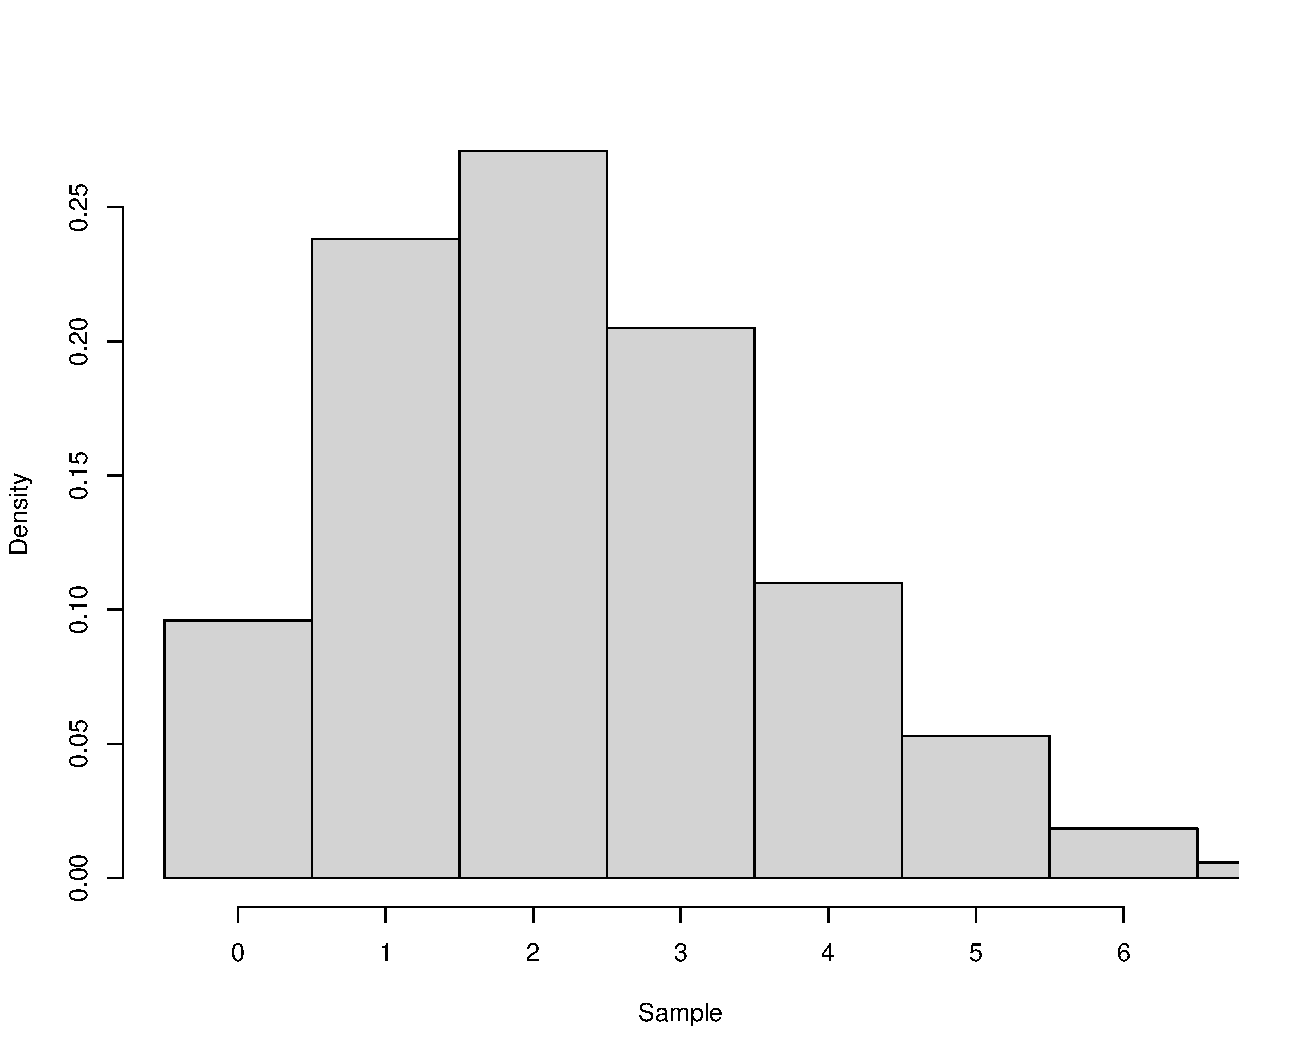
\includegraphics[width = 0.6\textwidth]{binlogsample}
		\caption{Промоделированное биномиально-логарифмическое распределение. $ q = 0.2, p = 0.25 $ и $ n = 8 $}
		\label{img:binlogsample}
	\end{figure}
	
	Напомним, что сложное распределение "--- это случайная сумма случайных величин, поэтому для моделирования выборки из $ n $ элементов этого распределения, нужно смоделировать выборку из $ n $ элементов первого простого распределения, обозначающего количество слагаемых, для каждого из которых вычисляется сумма смоделированной выборки из элементов второго, чьё количество равно значению элемента из первого.
	
	Функция, позволяющая моделировать биномиально-логарифмическое распределение в R:
	\begin{lstlisting}[language=R]
# Modeling of binomial-logarithmic distribution.
# sumlog - accumulated probabilities of the logarithmic
# distribution.
rbinomlog <- function(num = 1, sumlog, n = 1, p = 0.5) {
	res <- c()
	
	for(i in rbinom(num, n, p)){
		res <- c(res, sum(0, rnlog(i, sumlog)))
	}
	
	res
}
	\end{lstlisting}
	\label{page:Rmodel}
	Промоделированное биномиально-логарифмическое распределение с рассеянием меньше $ 1 $ представлено на рис. \ref{img:binlogsample}.
	
	\section{Оценка параметров и проверка согласия}
	
	Для оценки параметров применяется метод максимального правдоподобия, для чего, в первую очередь, составляется функция правдоподобия (пример приведём для биномиально-логарифмического распределения):
	
	\begin{lstlisting}[language=R]
m_log_lik_binomlog <- function(x.in, p = 0.5, n = 1, q = 0.5){
	if (q <= 0 || q >= 1 || p <= 0 || p >= 1 || n <= 0){
		return(-log(0));
	}
	
	-sum(sapply(x.in, function(i)
	 log(get_prob_binomlog(i, p, n, q))))
}
	\end{lstlisting}

	Часто приходится работать с частотами дискретных распределений, а не самой выборкой, поэтому для применения в функциях правдоподобия приведём функцию для создания выборки по частотам:
	
\begin{lstlisting}[language=R]
generate_sample <- function(num_k){
	rep.int(0:(length(num_k) - 1), num_k)
}
\end{lstlisting}	

	Тест $\chi ^2$ по умолчанию не умеет объединять состояния для улучшения применимости, поэтому напишем свою статистику:
	
\begin{lstlisting}[language=R]
my_chisq <- function(exp_prob, prob){
	sum((exp_prob - prob)^2 / prob)
}
\end{lstlisting}

	Теперь приведём основную функцию всей программы, которая производит оценку параметров, проверяет согласие и строит гистограмму:

\begin{lstlisting}[language=R]
hist_make <- function (n, exp_prob, get_hist, distr = 'binomlog'){
  sam <- generate_sample(exp_prob)
  N <- length(sam)
  var_sam <- var(sam) * (N - 1) / N
  mean_sam <- mean(sam)
  exp_prob <- exp_prob / N
	
  if (n == 0){
    df <- -1
  }
  else{
    df <- 0
  }

  # Estimation of parameters for different distributions
  # Binom-log
  if (distr == 'binomlog'){
  	# If the value of parameter n is set to zero,
  	# then its evaluation is also performed
    if (n == 0){
      left <- 1
      right <- 1000
      
      # The ternary search method
      while (right - left > 2) {
        nLeft <- (2 * left + right) %/% 3
        nRight <- (left + 2 * right) %/% 3

        qLeft <- optim(c(0.5, 1 / nLeft), function(x)
         m_log_lik_binomlog(sam, p = x[2], n = nLeft, q = x[1]))
        qRight <- optim(c(0.5, 1 / nRight), function(x)
         m_log_lik_binomlog(sam, p = x[2], n = nRight, q = x[1]))

        if (qLeft$value <= qRight$value) {
          right <- nRight
        }
        else{
          left <- nLeft
        }
      }

      minValue <- optim(c(0.5, 1 / (left + 1)), function(x)
      m_log_lik_binomlog(sam, p = x[2], n = left, q = x[1]))
      q <- minValue$par[1]
      p <- minValue$par[2]
      n <- left

      for (i in (left + 1):right){
        value <- optim(c(0.5, 1 / i), function(x)
         m_log_lik_binomlog(sam, p = x[2], n = i, q = x[1]))

      if (value$value <= minValue$value){
        minValue <- value
        q <- minValue$par[1]
        p <- minValue$par[2]
        n <- i
      }
    }
  }
  # If n is given, then the score is only p and q
  else {
    q <- optimize(function(x) 
     m_log_lik_binomlog(sam, p = (var_sam / mean_sam *
     log(1 - x) * (1 - x) - log(1 - x)) / x, n = n, q = x),
     c(0.01, 0.99))$minimum
    p <- (var_sam / mean_sam * log(1 - q) * (1 - q) -
     log(1 - q)) / q
  }

    res <- c(n, q, p)
  }
  # Log-binom
  else if (distr == 'logbinom'){
    if (n == 0){
      left <- 1
      right <- 1000

      while (right - left > 2) {
        nLeft <- (2 * left + right) %/% 3
        nRight <- (left + 2 * right) %/% 3

        qLeft <- optim(c(0.5, 1 / nLeft), function(x)
         m_log_lik_logbinom(sam, q = x[1], p = x[2], n = nLeft))
        qRight <- optim(c(0.5, 1 / nRight), function(x)
         m_log_lik_logbinom(sam, q = x[1], p = x[2], n = nRight))

        if (qLeft$value <= qRight$value) {
          right <- nRight
        }
        else{
          left <- nLeft
        }
      }

      minValue <- optim(c(0.5, 1 / (left + 1)), function(x)
       m_log_lik_logbinom(sam, q = x[1], p = x[2], n = left))
      q <- minValue$par[1]
      p <- minValue$par[2]
      n <- left

      for (i in (left + 1):right){
        value <- optim(c(0.5, 1 / i), function(x)
         m_log_lik_logbinom(sam, q = x[1], p = x[2], n = i))

        if (value$value <= minValue$value){
          minValue <- value
          q <- minValue$par[1]
          p <- minValue$par[2]
          n <- i
        }
      }
    }
    else {
      q <- optimize(function(x)
       m_log_lik_logbinom(sam, q = x, p = - log(1 - x) *
       (1 - x) / n / x * mean_sam, n = n),
       c(0.01, 0.99))$minimum
      p <- -log(1 - q) * (1 - q) / n / q * mean_sam
    }

    res <- c(n, q, p)
  # Log-pois
  } else if (distr == 'logpois'){
    q <- optim(c(0.5, 1), function(x) 
     m_log_lik_logpois(sam, q = x[1], lambda = x[2]))
    lambda <- q$par[2]
    q <- q$par[1]
    res <- c(lambda, q)
  # Negative binom
  } else if (distr == 'nbinom'){
    q <- optim(c(0.5, 1), function(x)
     m_log_lik_nbinom(sam, q = x[1], n = x[2]))
    n <- q$par[2]
    q <- q$par[1]
    res <- c(n, q)
  # The sum of two negative binomials
  } else if (distr == "doublenbinom"){
    q <- optim(c(0.8, 1, 0.5, 1),
     function(x) m_log_lik_doublenbinom(sam, p_1 = x[1],
     size_1 = x[2], p_2 = x[3], size_2 = x[4]))
    res <- c(q$par[1], q$par[2], q$par[3], q$par[4])
  }

  prob <- c()

  # Getting accurate probabilities based on estimates
  for (i in 0:(length(exp_prob) - 2)){
    if (distr == 'binomlog'){
      prob <- c(prob, get_prob_binomlog(i, p = res[3],
       n = res[1], q = res[2]))
    } else if (distr == 'logbinom'){
      prob <- c(prob, get_prob_logbinom(i, q = res[2],
       p = res[3], n = res[1]))
    } else if (distr == 'logpois'){
      prob <- c(prob, get_prob_logpois(i, q = res[2],
       lambda = res[1]))
    } else if (distr == 'nbinom'){
      prob <- c(prob, dnbinom(i, size = res[1],
       prob = res[2]))
    } else if (distr == 'doublenbinom'){
      prob <- c(prob, get_prob_doublenbinom(i, p_1 = res[1],
       size_1 = res[2], p_2 = res[3], size_2 = res[4]))
    }
  }

  prob <- c(prob, 1 - sum(prob))

  max_el_x = max(sam)
  max_el_y = max(exp_prob, prob)

  # Histogram on demand
  if (get_hist){
    hist.default(sam, probability = TRUE, breaks = seq(-0.5,
     max_el_x + 0.5, 1), xlim = c(-0.5, max_el_x + 0.5),
     ylim = c(0, max_el_y), xlab = "Sample", main = "")
    points(0:(length(prob) - 1), prob)
  }

  # Combining states
  for (i in 1:length(prob)){
    while (100 * prob[i] < 5 && i < length(prob)){
      prob[i] <- prob[i] + prob[i + 1]
      prob <- prob[-(i + 1)]
      exp_prob[i] <- exp_prob[i] + exp_prob[i + 1]
      exp_prob <- exp_prob[-(i + 1)]
    }
  }
	
  if (100 * prob[length(prob)] < 5){
    prob[length(prob) - 1] <- prob[length(prob) - 1] +
     prob[length(prob)]
    prob <- prob[-length(prob)]
    exp_prob[length(exp_prob) - 1] <-
     exp_prob[length(exp_prob) - 1] + exp_prob[length(exp_prob)]
    exp_prob <- exp_prob[-length(exp_prob)]
  }
	
  # Counting degrees of freedom
  df <- df + length(prob) - 3
	
  if (df < 1){
    df <- 1
  }
	
  # Chi Square test
  chi <- N * my_chisq(exp_prob, prob)
  res <- c(res, 1 - pchisq(chi, df))
	
  res
}
	\end{lstlisting}
\end{document}